\documentclass[twoside]{book}

% Packages required by doxygen
\usepackage{fixltx2e}
\usepackage{calc}
\usepackage{doxygen}
\usepackage[export]{adjustbox} % also loads graphicx
\usepackage{graphicx}
\usepackage[utf8]{inputenc}
\usepackage{makeidx}
\usepackage{multicol}
\usepackage{multirow}
\PassOptionsToPackage{warn}{textcomp}
\usepackage{textcomp}
\usepackage[nointegrals]{wasysym}
\usepackage[table]{xcolor}

% Font selection
\usepackage[T1]{fontenc}
\usepackage[scaled=.90]{helvet}
\usepackage{courier}
\usepackage{amssymb}
\usepackage{sectsty}
\renewcommand{\familydefault}{\sfdefault}
\allsectionsfont{%
  \fontseries{bc}\selectfont%
  \color{darkgray}%
}
\renewcommand{\DoxyLabelFont}{%
  \fontseries{bc}\selectfont%
  \color{darkgray}%
}
\newcommand{\+}{\discretionary{\mbox{\scriptsize$\hookleftarrow$}}{}{}}

% Page & text layout
\usepackage{geometry}
\geometry{%
  a4paper,%
  top=2.5cm,%
  bottom=2.5cm,%
  left=2.5cm,%
  right=2.5cm%
}
\tolerance=750
\hfuzz=15pt
\hbadness=750
\setlength{\emergencystretch}{15pt}
\setlength{\parindent}{0cm}
\setlength{\parskip}{3ex plus 2ex minus 2ex}
\makeatletter
\renewcommand{\paragraph}{%
  \@startsection{paragraph}{4}{0ex}{-1.0ex}{1.0ex}{%
    \normalfont\normalsize\bfseries\SS@parafont%
  }%
}
\renewcommand{\subparagraph}{%
  \@startsection{subparagraph}{5}{0ex}{-1.0ex}{1.0ex}{%
    \normalfont\normalsize\bfseries\SS@subparafont%
  }%
}
\makeatother

% Headers & footers
\usepackage{fancyhdr}
\pagestyle{fancyplain}
\fancyhead[LE]{\fancyplain{}{\bfseries\thepage}}
\fancyhead[CE]{\fancyplain{}{}}
\fancyhead[RE]{\fancyplain{}{\bfseries\leftmark}}
\fancyhead[LO]{\fancyplain{}{\bfseries\rightmark}}
\fancyhead[CO]{\fancyplain{}{}}
\fancyhead[RO]{\fancyplain{}{\bfseries\thepage}}
\fancyfoot[LE]{\fancyplain{}{}}
\fancyfoot[CE]{\fancyplain{}{}}
\fancyfoot[RE]{\fancyplain{}{\bfseries\scriptsize Generated by Doxygen }}
\fancyfoot[LO]{\fancyplain{}{\bfseries\scriptsize Generated by Doxygen }}
\fancyfoot[CO]{\fancyplain{}{}}
\fancyfoot[RO]{\fancyplain{}{}}
\renewcommand{\footrulewidth}{0.4pt}
\renewcommand{\chaptermark}[1]{%
  \markboth{#1}{}%
}
\renewcommand{\sectionmark}[1]{%
  \markright{\thesection\ #1}%
}

% Indices & bibliography
\usepackage{natbib}
\usepackage[titles]{tocloft}
\setcounter{tocdepth}{3}
\setcounter{secnumdepth}{5}
\makeindex

% Hyperlinks (required, but should be loaded last)
\usepackage{ifpdf}
\ifpdf
  \usepackage[pdftex,pagebackref=true]{hyperref}
\else
  \usepackage[ps2pdf,pagebackref=true]{hyperref}
\fi
\hypersetup{%
  colorlinks=true,%
  linkcolor=blue,%
  citecolor=blue,%
  unicode%
}

% Custom commands
\newcommand{\clearemptydoublepage}{%
  \newpage{\pagestyle{empty}\cleardoublepage}%
}

\usepackage{caption}
\captionsetup{labelsep=space,justification=centering,font={bf},singlelinecheck=off,skip=4pt,position=top}

%===== C O N T E N T S =====

\begin{document}

% Titlepage & ToC
\hypersetup{pageanchor=false,
             bookmarksnumbered=true,
             pdfencoding=unicode
            }
\pagenumbering{alph}
\begin{titlepage}
\vspace*{7cm}
\begin{center}%
{\Large Q-\/a\+Rt Encoder \\[1ex]\large Revision 1 }\\
\vspace*{1cm}
{\large Generated by Doxygen 1.8.12}\\
\end{center}
\end{titlepage}
\clearemptydoublepage
\pagenumbering{roman}
\tableofcontents
\clearemptydoublepage
\pagenumbering{arabic}
\hypersetup{pageanchor=true}

%--- Begin generated contents ---
\chapter{Mainpage}
\label{index}\hypertarget{index}{}\input{index}
\chapter{Q-\/a\+Rt Code Source Code}
\label{md__r_e_a_d_m_e}
\hypertarget{md__r_e_a_d_m_e}{}
\input{md__r_e_a_d_m_e}
\chapter{Hierarchical Index}
\section{Class Hierarchy}
This inheritance list is sorted roughly, but not completely, alphabetically\+:\begin{DoxyCompactList}
\item Frame\begin{DoxyCompactList}
\item \contentsline{section}{G\+U\+I.\+Application}{\pageref{class_g_u_i_1_1_application}}{}
\end{DoxyCompactList}
\end{DoxyCompactList}

\chapter{Class Index}
\section{Class List}
Here are the classes, structs, unions and interfaces with brief descriptions\+:\begin{DoxyCompactList}
\item\contentsline{section}{\hyperlink{class_g_u_i_1_1_application}{G\+U\+I.\+Application} }{\pageref{class_g_u_i_1_1_application}}{}
\end{DoxyCompactList}

\chapter{File Index}
\section{File List}
Here is a list of all documented files with brief descriptions\+:\begin{DoxyCompactList}
\item\contentsline{section}{\hyperlink{_constant_8py}{Constant.\+py} \\*Constant }{\pageref{_constant_8py}}{}
\item\contentsline{section}{\hyperlink{_data_8py}{Data.\+py} \\*Data }{\pageref{_data_8py}}{}
\item\contentsline{section}{\hyperlink{_draw_8py}{Draw.\+py} \\*Draw }{\pageref{_draw_8py}}{}
\item\contentsline{section}{\hyperlink{_e_c_c_8py}{E\+C\+C.\+py} \\*E\+CC }{\pageref{_e_c_c_8py}}{}
\item\contentsline{section}{\hyperlink{_main_8py}{Main.\+py} \\*Main }{\pageref{_main_8py}}{}
\item\contentsline{section}{\hyperlink{_matrix_8py}{Matrix.\+py} \\*Matrix }{\pageref{_matrix_8py}}{}
\item\contentsline{section}{\hyperlink{_structure_8py}{Structure.\+py} \\*Structure }{\pageref{_structure_8py}}{}
\end{DoxyCompactList}

\chapter{Class Documentation}
\hypertarget{class_g_u_i_1_1_application}{}\section{G\+U\+I.\+Application Class Reference}
\label{class_g_u_i_1_1_application}\index{G\+U\+I.\+Application@{G\+U\+I.\+Application}}
Inheritance diagram for G\+U\+I.\+Application\+:\begin{figure}[H]
\begin{center}
\leavevmode
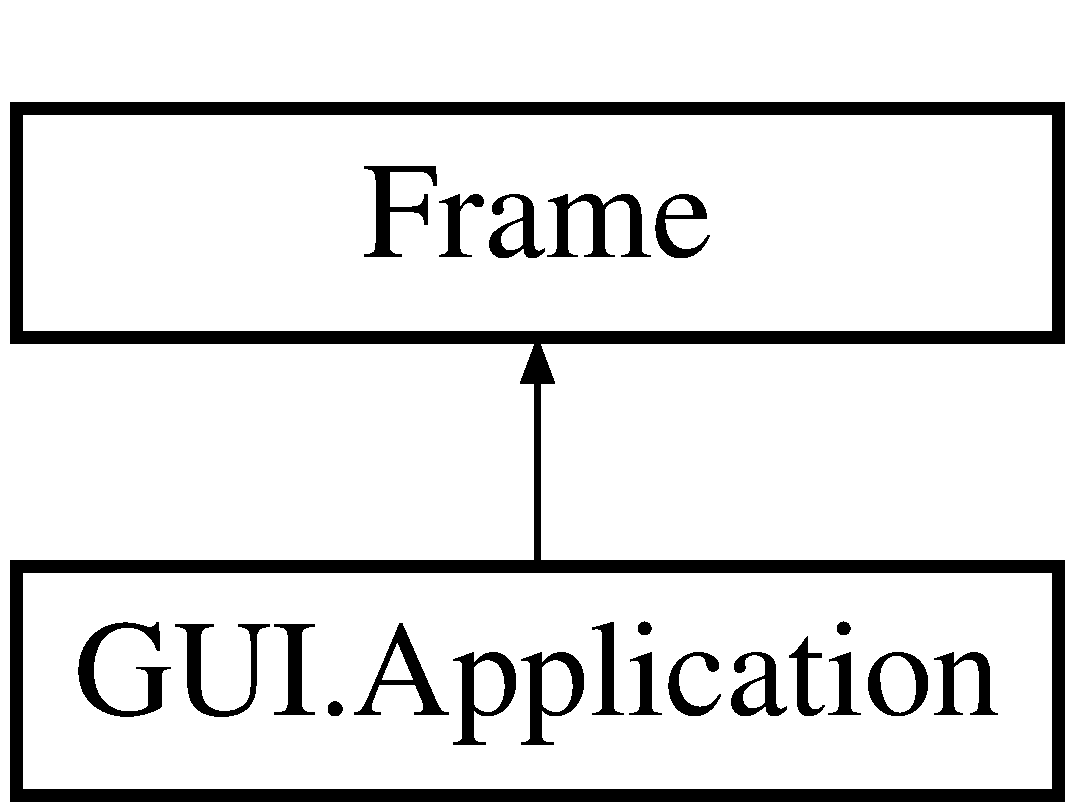
\includegraphics[height=2.000000cm]{class_g_u_i_1_1_application}
\end{center}
\end{figure}
\subsection*{Public Member Functions}
\begin{DoxyCompactItemize}
\item 
\hypertarget{class_g_u_i_1_1_application_a66fd072a15ec95d3c778c10c1484961a}{}\label{class_g_u_i_1_1_application_a66fd072a15ec95d3c778c10c1484961a} 
def \hyperlink{class_g_u_i_1_1_application_a66fd072a15ec95d3c778c10c1484961a}{\+\_\+\+\_\+init\+\_\+\+\_\+} (self, master)
\begin{DoxyCompactList}\small\item\em constructor for G\+UI \end{DoxyCompactList}\item 
def \hyperlink{class_g_u_i_1_1_application_a84a6c38f860f505a4bb7a0356393d24a}{create\+\_\+widgets} (self)
\begin{DoxyCompactList}\small\item\em Method to create all G\+UI widgets. \end{DoxyCompactList}\item 
\hypertarget{class_g_u_i_1_1_application_a25e3c2fd5e8bd6714c49930806f8a362}{}\label{class_g_u_i_1_1_application_a25e3c2fd5e8bd6714c49930806f8a362} 
def {\bfseries reveal} (self)
\end{DoxyCompactItemize}
\subsection*{Public Attributes}
\begin{DoxyCompactItemize}
\item 
\hypertarget{class_g_u_i_1_1_application_a78a10ff27558f6cdd52e4b9c234e4d4c}{}\label{class_g_u_i_1_1_application_a78a10ff27558f6cdd52e4b9c234e4d4c} 
{\bfseries photo}
\item 
\hypertarget{class_g_u_i_1_1_application_a1b09350b39cb79ae160a65d93e3e7dd5}{}\label{class_g_u_i_1_1_application_a1b09350b39cb79ae160a65d93e3e7dd5} 
{\bfseries logo}
\item 
\hypertarget{class_g_u_i_1_1_application_aa554ce58739d4315465f6b8e8e29c833}{}\label{class_g_u_i_1_1_application_aa554ce58739d4315465f6b8e8e29c833} 
{\bfseries instruction}
\item 
\hypertarget{class_g_u_i_1_1_application_ab0b9b7acf4e20c16939b96502d451e42}{}\label{class_g_u_i_1_1_application_ab0b9b7acf4e20c16939b96502d451e42} 
{\bfseries words}
\item 
\hypertarget{class_g_u_i_1_1_application_a944ea9c24a7b51ccc67c7260bacf3509}{}\label{class_g_u_i_1_1_application_a944ea9c24a7b51ccc67c7260bacf3509} 
{\bfseries version}
\item 
\hypertarget{class_g_u_i_1_1_application_a68e2325444ac25875d15bda0048e5523}{}\label{class_g_u_i_1_1_application_a68e2325444ac25875d15bda0048e5523} 
{\bfseries level}
\item 
\hypertarget{class_g_u_i_1_1_application_a10b21193562925e7831158eafa70c4e6}{}\label{class_g_u_i_1_1_application_a10b21193562925e7831158eafa70c4e6} 
{\bfseries picture}
\item 
\hypertarget{class_g_u_i_1_1_application_ae47d60f1396b8eccaee95f8a637dc5d7}{}\label{class_g_u_i_1_1_application_ae47d60f1396b8eccaee95f8a637dc5d7} 
{\bfseries col\+Var}
\item 
\hypertarget{class_g_u_i_1_1_application_ad876d4f8950f7fdeb15d97f122c2933c}{}\label{class_g_u_i_1_1_application_ad876d4f8950f7fdeb15d97f122c2933c} 
{\bfseries colorized}
\item 
\hypertarget{class_g_u_i_1_1_application_aaa386bfc5e1de14c43374e4be4722f9a}{}\label{class_g_u_i_1_1_application_aaa386bfc5e1de14c43374e4be4722f9a} 
{\bfseries contrast}
\item 
\hypertarget{class_g_u_i_1_1_application_abe9547b7045adde858aae8580fff9394}{}\label{class_g_u_i_1_1_application_abe9547b7045adde858aae8580fff9394} 
{\bfseries brightness}
\item 
\hypertarget{class_g_u_i_1_1_application_a35eea9f845d3eee6d188190fe4c682c6}{}\label{class_g_u_i_1_1_application_a35eea9f845d3eee6d188190fe4c682c6} 
{\bfseries name}
\item 
\hypertarget{class_g_u_i_1_1_application_a691bc2af89347b10b85484e2e5788ab3}{}\label{class_g_u_i_1_1_application_a691bc2af89347b10b85484e2e5788ab3} 
{\bfseries directory}
\end{DoxyCompactItemize}
\subsection*{Static Public Attributes}
\begin{DoxyCompactItemize}
\item 
\hypertarget{class_g_u_i_1_1_application_a6a8ca3a5882888d349cdedc911d175c2}{}\label{class_g_u_i_1_1_application_a6a8ca3a5882888d349cdedc911d175c2} 
{\bfseries button1}
\item 
\hypertarget{class_g_u_i_1_1_application_a90c619c846c3cea133c48377d4a4228d}{}\label{class_g_u_i_1_1_application_a90c619c846c3cea133c48377d4a4228d} 
{\bfseries self}
\item 
\hypertarget{class_g_u_i_1_1_application_ac13dddd2ea333e0d578157201347c34e}{}\label{class_g_u_i_1_1_application_ac13dddd2ea333e0d578157201347c34e} 
{\bfseries text}
\item 
\hypertarget{class_g_u_i_1_1_application_a5f870ca4bff8c0dfb37ddb5d307babb1}{}\label{class_g_u_i_1_1_application_a5f870ca4bff8c0dfb37ddb5d307babb1} 
{\bfseries width}
\item 
\hypertarget{class_g_u_i_1_1_application_a31931931fb7c0b4bae77306bcf5850c2}{}\label{class_g_u_i_1_1_application_a31931931fb7c0b4bae77306bcf5850c2} 
{\bfseries command}
\item 
\hypertarget{class_g_u_i_1_1_application_a84d12d24908d69fac56c33e65e5a7012}{}\label{class_g_u_i_1_1_application_a84d12d24908d69fac56c33e65e5a7012} 
{\bfseries reveal}
\item 
\hypertarget{class_g_u_i_1_1_application_a439307e042d5ce4cd154222b1d480f4e}{}\label{class_g_u_i_1_1_application_a439307e042d5ce4cd154222b1d480f4e} 
{\bfseries bg}
\item 
\hypertarget{class_g_u_i_1_1_application_a558223dab4a1a30fbf9b3562b4a51494}{}\label{class_g_u_i_1_1_application_a558223dab4a1a30fbf9b3562b4a51494} 
{\bfseries fg}
\item 
\hypertarget{class_g_u_i_1_1_application_ad9d9221e2a899fe408e2d8e6796f32f2}{}\label{class_g_u_i_1_1_application_ad9d9221e2a899fe408e2d8e6796f32f2} 
{\bfseries font}
\end{DoxyCompactItemize}


\subsection{Detailed Description}
\begin{DoxyVerb}A Gui App \end{DoxyVerb}
 

\subsection{Member Function Documentation}
\hypertarget{class_g_u_i_1_1_application_a84a6c38f860f505a4bb7a0356393d24a}{}\label{class_g_u_i_1_1_application_a84a6c38f860f505a4bb7a0356393d24a} 
\index{G\+U\+I\+::\+Application@{G\+U\+I\+::\+Application}!create\+\_\+widgets@{create\+\_\+widgets}}
\index{create\+\_\+widgets@{create\+\_\+widgets}!G\+U\+I\+::\+Application@{G\+U\+I\+::\+Application}}
\subsubsection{\texorpdfstring{create\+\_\+widgets()}{create\_widgets()}}
{\footnotesize\ttfamily def G\+U\+I.\+Application.\+create\+\_\+widgets (\begin{DoxyParamCaption}\item[{}]{self }\end{DoxyParamCaption})}



Method to create all G\+UI widgets. 

Creates the predefined widgets necessary for program operation. \begin{DoxyReturn}{Returns}
None 
\end{DoxyReturn}


The documentation for this class was generated from the following file\+:\begin{DoxyCompactItemize}
\item 
\hyperlink{_g_u_i_8py}{G\+U\+I.\+py}\end{DoxyCompactItemize}

\chapter{File Documentation}
\hypertarget{_constant_8py}{}\section{Constant.\+py File Reference}
\label{_constant_8py}\index{Constant.\+py@{Constant.\+py}}


Constant  


\subsection*{Variables}
\begin{DoxyCompactItemize}
\item 
dictionary {\bfseries Constant.\+char\+\_\+cap}
\item 
\hypertarget{_constant_8py_a79379c282cf67fcf44ff4b5a2a601e0e}{}\label{_constant_8py_a79379c282cf67fcf44ff4b5a2a601e0e} 
dictionary {\bfseries Constant.\+mindex} = \{\textquotesingle{}numeric\textquotesingle{}\+:0, \textquotesingle{}alphanumeric\textquotesingle{}\+:1, \textquotesingle{}byte\textquotesingle{}\+:2, \textquotesingle{}kanji\textquotesingle{}\+:3\}
\item 
list {\bfseries Constant.\+required\+\_\+bytes}
\item 
\hypertarget{_constant_8py_a5aacb8cedd7e787df1f63baf58d853cb}{}\label{_constant_8py_a5aacb8cedd7e787df1f63baf58d853cb} 
string {\bfseries Constant.\+num\+\_\+list} = \textquotesingle{}0123456789\textquotesingle{}
\item 
\hypertarget{_constant_8py_aa8854b061d2169a4d089108bd0e90189}{}\label{_constant_8py_aa8854b061d2169a4d089108bd0e90189} 
string {\bfseries Constant.\+alphanum\+\_\+list} = \textquotesingle{}0123456789\+A\+B\+C\+D\+E\+F\+G\+H\+I\+J\+K\+L\+M\+N\+O\+P\+Q\+R\+S\+T\+U\+V\+W\+X\+Y\+Z \$\%$\ast$+-\/./\+:\textquotesingle{}
\item 
list {\bfseries Constant.\+grouping\+\_\+list}
\item 
\hypertarget{_constant_8py_af5754cb0c5a752e6dca251a34af0c8a5}{}\label{_constant_8py_af5754cb0c5a752e6dca251a34af0c8a5} 
dictionary {\bfseries Constant.\+mode\+\_\+indicator} = \{\textquotesingle{}numeric\textquotesingle{}\+: \textquotesingle{}0001\textquotesingle{}, \textquotesingle{}alphanumeric\textquotesingle{}\+: \textquotesingle{}0010\textquotesingle{}, \textquotesingle{}byte\textquotesingle{}\+: \textquotesingle{}0100\textquotesingle{}, \textquotesingle{}kanji\textquotesingle{}\+: \textquotesingle{}1000\textquotesingle{}\}
\item 
dictionary {\bfseries Constant.\+G\+P\+\_\+list}
\item 
list {\bfseries Constant.\+ecc\+\_\+num\+\_\+per\+\_\+block}
\item 
list {\bfseries Constant.\+po2}
\item 
list {\bfseries Constant.\+log}
\item 
\hypertarget{_constant_8py_a6884b5cf804ad44fad68bb9a4637dd85}{}\label{_constant_8py_a6884b5cf804ad44fad68bb9a4637dd85} 
dictionary {\bfseries Constant.\+lindex} = \{\textquotesingle{}L\textquotesingle{}\+:0, \textquotesingle{}M\textquotesingle{}\+:1, \textquotesingle{}Q\textquotesingle{}\+:2, \textquotesingle{}H\textquotesingle{}\+:3\}
\item 
\hypertarget{_constant_8py_a530e316d9bce1704055c23cca4277454}{}\label{_constant_8py_a530e316d9bce1704055c23cca4277454} 
tuple {\bfseries Constant.\+required\+\_\+remainder\+\_\+bits} = (0,7,7,7,7,7,0,0,0,0,0,0,0,3,3,3,3,3,3,3,4,4,4,4,4,4,4,3,3,3,3,3,3,3,0,0,0,0,0,0)
\item 
list {\bfseries Constant.\+alig\+\_\+location}
\item 
list {\bfseries Constant.\+format\+\_\+info\+\_\+str}
\item 
list {\bfseries Constant.\+version\+\_\+info\+\_\+str}
\end{DoxyCompactItemize}


\subsection{Detailed Description}
Constant 

\begin{DoxyDate}{Date}
13/11/2016 This class contains useful constants for qr processing.
\end{DoxyDate}
Module is taken from original project. Contains useful constants for QR code computation.~\newline
 State variables\+:~\newline
 char\+\_\+cap -\/ list of character capacities for each version and error correction level~\newline
 required\+\_\+bytes -\/ list of required bytes for each version~\newline
 num\+\_\+list -\/ list of valid characters for numeric mode~\newline
 alphanum\+\_\+list -\/ list of valid characters for alphanumeric mode~\newline
 grouping\+\_\+list -\/ list of codeword grouping into blocks for each version~\newline
 mode\+\_\+indicator -\/ list of encoding mode strings~\newline
 G\+P\+\_\+list -\/ lsit of generator polynomials~\newline
 ecc\+\_\+num\+\_\+per\+\_\+block -\/ list of error correction codewords per block for each version and error correction level~\newline
 po2 -\/ list of powers of two in Galois Field~\newline
 log -\/ list of logarithms in Galois Field~\newline
 required\+\_\+remainder\+\_\+bits -\/ list of required remainder bits for each version for interleaving~\newline
 alig\+\_\+location -\/ list of alignment pattern locations for each version~\newline
 format\+\_\+info\+\_\+string -\/ list of format strings for each mask pattern~\newline
 version\+\_\+info\+\_\+string -\/ list of version strings for each version~\newline
 

\subsection{Variable Documentation}
\hypertarget{_constant_8py_file_a3b6d358ff4f208366241447d413be8db}{}\label{_constant_8py_file_a3b6d358ff4f208366241447d413be8db} 
\index{Constant.\+py@{Constant.\+py}!alig\+\_\+location@{alig\+\_\+location}}
\index{alig\+\_\+location@{alig\+\_\+location}!Constant.\+py@{Constant.\+py}}
\subsubsection{\texorpdfstring{alig\+\_\+location}{alig\_location}}
{\footnotesize\ttfamily list Constant.\+alig\+\_\+location}

{\bfseries Initial value\+:}
\begin{DoxyCode}
1 =  [
2     (6, 18), (6, 22), (6, 26), (6, 30), (6, 34), (6, 22, 38), (6, 24, 42), (6, 26, 46), (6, 28, 50), (6, 30
      , 54), (6, 32, 58), (6, 34, 62), (6, 26, 46, 66), (6, 26, 48, 70), (6, 26, 50, 74), (6, 30, 54, 78), (6, 30,
       56, 82), (6, 30, 58, 86), (6, 34, 62, 90), (6, 28, 50, 72, 94), (6, 26, 50, 74, 98), (6, 30, 54, 78, 102), 
      (6, 28, 54, 80, 106), (6, 32, 58, 84, 110), (6, 30, 58, 86, 114), (6, 34, 62, 90, 118), (6, 26, 50, 74, 98, 
      122), (6, 30, 54, 78, 102, 126), (6, 26, 52, 78, 104, 130), (6, 30, 56, 82, 108, 134), (6, 34, 60, 86, 112, 
      138), (6, 30, 58, 86, 114, 142), (6, 34, 62, 90, 118, 146), (6, 30, 54, 78, 102, 126, 150), (6, 24, 50, 76, 
      102, 128, 154), (6, 28, 54, 80, 106, 132, 158), (6, 32, 58, 84, 110, 136, 162), (6, 26, 54, 82, 110, 138, 16
      6), (6, 30, 58, 86, 114, 142, 170)
3     ]
\end{DoxyCode}
\hypertarget{_constant_8py_file_a2941b2e867750c768f4df9a6fbb9989e}{}\label{_constant_8py_file_a2941b2e867750c768f4df9a6fbb9989e} 
\index{Constant.\+py@{Constant.\+py}!char\+\_\+cap@{char\+\_\+cap}}
\index{char\+\_\+cap@{char\+\_\+cap}!Constant.\+py@{Constant.\+py}}
\subsubsection{\texorpdfstring{char\+\_\+cap}{char\_cap}}
{\footnotesize\ttfamily dictionary Constant.\+char\+\_\+cap}

{\bfseries Initial value\+:}
\begin{DoxyCode}
1 =  \{
2         \textcolor{stringliteral}{'L'}: [(41, 25, 17, 10), (77, 47, 32, 20), (127, 77, 53, 32), (187, 114, 78, 48), (255, 154, 106, 65
      ), (322, 195, 134, 82), (370, 224, 154, 95), (461, 279, 192, 118), (552, 335, 230, 141), (652, 395, 271, 167
      ), (772, 468, 321, 198), (883, 535, 367, 226), (1022, 619, 425, 262), (1101, 667, 458, 282), (1250, 758, 520
      , 320), (1408, 854, 586, 361), (1548, 938, 644, 397), (1725, 1046, 718, 442), (1903, 1153, 792, 488), (2061,
       1249, 858, 528), (2232, 1352, 929, 572), (2409, 1460, 1003, 618), (2620, 1588, 1091, 672), (2812, 1704, 117
      1, 721), (3057, 1853, 1273, 784), (3283, 1990, 1367, 842), (3517, 2132, 1465, 902), (3669, 2223, 1528, 940),
       (3909, 2369, 1628, 1002), (4158, 2520, 1732, 1066), (4417, 2677, 1840, 1132), (4686, 2840, 1952, 1201), (49
      65, 3009, 2068, 1273), (5253, 3183, 2188, 1347), (5529, 3351, 2303, 1417), (5836, 3537, 2431, 1496), (6153, 
      3729, 2563, 1577), (6479, 3927, 2699, 1661), (6743, 4087, 2809, 1729), (7089, 4296, 2953, 1817)],
3         \textcolor{stringliteral}{'M'}: [(34, 20, 14, 8), (63, 38, 26, 16), (101, 61, 42, 26), (149, 90, 62, 38), (202, 122, 84, 52), 
      (255, 154, 106, 65), (293, 178, 122, 75), (365, 221, 152, 93), (432, 262, 180, 111), (513, 311, 213, 131), (
      604, 366, 251, 155), (691, 419, 287, 177), (796, 483, 331, 204), (871, 528, 362, 223), (991, 600, 412, 254),
       (1082, 656, 450, 277), (1212, 734, 504, 310), (1346, 816, 560, 345), (1500, 909, 624, 384), (1600, 970, 666
      , 410), (1708, 1035, 711, 438), (1872, 1134, 779, 480), (2059, 1248, 857, 528), (2188, 1326, 911, 561), (239
      5, 1451, 997, 614), (2544, 1542, 1059, 652), (2701, 1637, 1125, 692), (2857, 1732, 1190, 732), (3035, 1839, 
      1264, 778), (3289, 1994, 1370, 843), (3486, 2113, 1452, 894), (3693, 2238, 1538, 947), (3909, 2369, 1628, 10
      02), (4134, 2506, 1722, 1060), (4343, 2632, 1809, 1113), (4588, 2780, 1911, 1176), (4775, 2894, 1989, 1224),
       (5039, 3054, 2099, 1292), (5313, 3220, 2213, 1362), (5596, 3391, 2331, 1435)],
4         \textcolor{stringliteral}{'Q'}: [(27, 16, 11, 7), (48, 29, 20, 12), (77, 47, 32, 20), (111, 67, 46, 28), (144, 87, 60, 37), (1
      78, 108, 74, 45), (207, 125, 86, 53), (259, 157, 108, 66), (312, 189, 130, 80), (364, 221, 151, 93), (427, 2
      59, 177, 109), (489, 296, 203, 125), (580, 352, 241, 149), (621, 376, 258, 159), (703, 426, 292, 180), (775,
       470, 322, 198), (876, 531, 364, 224), (948, 574, 394, 243), (1063, 644, 442, 272), (1159, 702, 482, 297), (
      1224, 742, 509, 314), (1358, 823, 565, 348), (1468, 890, 611, 376), (1588, 963, 661, 407), (1718, 1041, 715,
       440), (1804, 1094, 751, 462), (1933, 1172, 805, 496), (2085, 1263, 868, 534), (2181, 1322, 908, 559), (2358
      , 1429, 982, 604), (2473, 1499, 1030, 634), (2670, 1618, 1112, 684), (2805, 1700, 1168, 719), (2949, 1787, 1
      228, 756), (3081, 1867, 1283, 790), (3244, 1966, 1351, 832), (3417, 2071, 1423, 876), (3599, 2181, 1499, 923
      ), (3791, 2298, 1579, 972), (3993, 2420, 1663, 1024)],
5         \textcolor{stringliteral}{'H'}: [(17, 10, 7, 4), (34, 20, 14, 8), (58, 35, 24, 15), (82, 50, 34, 21), (106, 64, 44, 27), (139,
       84, 58, 36), (154, 93, 64, 39), (202, 122, 84, 52), (235, 143, 98, 60), (288, 174, 119, 74), (331, 200, 137
      , 85), (374, 227, 155, 96), (427, 259, 177, 109), (468, 283, 194, 120), (530, 321, 220, 136), (602, 365, 250
      , 154), (674, 408, 280, 173), (746, 452, 310, 191), (813, 493, 338, 208), (919, 557, 382, 235), (969, 587, 4
      03, 248), (1056, 640, 439, 270), (1108, 672, 461, 284), (1228, 744, 511, 315), (1286, 779, 535, 330), (1425,
       864, 593, 365), (1501, 910, 625, 385), (1581, 958, 658, 405), (1677, 1016, 698, 430), (1782, 1080, 742, 457
      ), (1897, 1150, 790, 486), (2022, 1226, 842, 518), (2157, 1307, 898, 553), (2301, 1394, 958, 590), (2361, 14
      31, 983, 605), (2524, 1530, 1051, 647), (2625, 1591, 1093, 673), (2735, 1658, 1139, 701), (2927, 1774, 1219,
       750), (3057, 1852, 1273, 784)]
6         \}
\end{DoxyCode}
\hypertarget{_constant_8py_file_a49b20252ab414381deff5245456296e3}{}\label{_constant_8py_file_a49b20252ab414381deff5245456296e3} 
\index{Constant.\+py@{Constant.\+py}!ecc\+\_\+num\+\_\+per\+\_\+block@{ecc\+\_\+num\+\_\+per\+\_\+block}}
\index{ecc\+\_\+num\+\_\+per\+\_\+block@{ecc\+\_\+num\+\_\+per\+\_\+block}!Constant.\+py@{Constant.\+py}}
\subsubsection{\texorpdfstring{ecc\+\_\+num\+\_\+per\+\_\+block}{ecc\_num\_per\_block}}
{\footnotesize\ttfamily list Constant.\+ecc\+\_\+num\+\_\+per\+\_\+block}

{\bfseries Initial value\+:}
\begin{DoxyCode}
1 =  [
2     (7, 10, 13, 17), (10, 16, 22, 28), (15, 26, 18, 22), (20, 18, 26, 16), (26, 24, 18, 22), (18, 16, 24, 2
      8), (20, 18, 18, 26), (24, 22, 22, 26), (30, 22, 20, 24), (18, 26, 24, 28), (20, 30, 28, 24), (24, 22, 26, 2
      8), (26, 22, 24, 22), (30, 24, 20, 24), (22, 24, 30, 24), (24, 28, 24, 30), (28, 28, 28, 28), (30, 26, 28, 2
      8), (28, 26, 26, 26), (28, 26, 30, 28), (28, 26, 28, 30), (28, 28, 30, 24), (30, 28, 30, 30), (30, 28, 30, 3
      0), (26, 28, 30, 30), (28, 28, 28, 30), (30, 28, 30, 30), (30, 28, 30, 30), (30, 28, 30, 30), (30, 28, 30, 3
      0), (30, 28, 30, 30), (30, 28, 30, 30), (30, 28, 30, 30), (30, 28, 30, 30), (30, 28, 30, 30), (30, 28, 30, 3
      0), (30, 28, 30, 30), (30, 28, 30, 30), (30, 28, 30, 30), (30, 28, 30, 30)
3     ]
\end{DoxyCode}
\hypertarget{_constant_8py_file_a610258b49619e158a9e6b023ccf45bcd}{}\label{_constant_8py_file_a610258b49619e158a9e6b023ccf45bcd} 
\index{Constant.\+py@{Constant.\+py}!format\+\_\+info\+\_\+str@{format\+\_\+info\+\_\+str}}
\index{format\+\_\+info\+\_\+str@{format\+\_\+info\+\_\+str}!Constant.\+py@{Constant.\+py}}
\subsubsection{\texorpdfstring{format\+\_\+info\+\_\+str}{format\_info\_str}}
{\footnotesize\ttfamily list Constant.\+format\+\_\+info\+\_\+str}

{\bfseries Initial value\+:}
\begin{DoxyCode}
1 =  [
2     [\textcolor{stringliteral}{'111011111000100'}, \textcolor{stringliteral}{'111001011110011'}, \textcolor{stringliteral}{'111110110101010'}, \textcolor{stringliteral}{'111100010011101'}, \textcolor{stringliteral}{'110011000101111'}, \textcolor{stringliteral}{'
      110001100011000'}, \textcolor{stringliteral}{'110110001000001'}, \textcolor{stringliteral}{'110100101110110'}], [\textcolor{stringliteral}{'101010000010010'}, \textcolor{stringliteral}{'101000100100101'}, \textcolor{stringliteral}{'101111001111100'},
       \textcolor{stringliteral}{'101101101001011'}, \textcolor{stringliteral}{'100010111111001'}, \textcolor{stringliteral}{'100000011001110'}, \textcolor{stringliteral}{'100111110010111'}, \textcolor{stringliteral}{'100101010100000'}], [\textcolor{stringliteral}{'
      011010101011111'}, \textcolor{stringliteral}{'011000001101000'}, \textcolor{stringliteral}{'011111100110001'}, \textcolor{stringliteral}{'011101000000110'}, \textcolor{stringliteral}{'010010010110100'}, \textcolor{stringliteral}{'010000110000011'}, \textcolor{stringliteral}{'
      010111011011010'}, \textcolor{stringliteral}{'010101111101101'}], [\textcolor{stringliteral}{'001011010001001'}, \textcolor{stringliteral}{'001001110111110'}, \textcolor{stringliteral}{'001110011100111'}, \textcolor{stringliteral}{'
      001100111010000'}, \textcolor{stringliteral}{'000011101100010'}, \textcolor{stringliteral}{'000001001010101'}, \textcolor{stringliteral}{'000110100001100'}, \textcolor{stringliteral}{'000100000111011'}]
3     ]
\end{DoxyCode}
\hypertarget{_constant_8py_file_addd6ab040c284fbee266709ba15f151b}{}\label{_constant_8py_file_addd6ab040c284fbee266709ba15f151b} 
\index{Constant.\+py@{Constant.\+py}!G\+P\+\_\+list@{G\+P\+\_\+list}}
\index{G\+P\+\_\+list@{G\+P\+\_\+list}!Constant.\+py@{Constant.\+py}}
\subsubsection{\texorpdfstring{G\+P\+\_\+list}{GP\_list}}
{\footnotesize\ttfamily dictionary Constant.\+G\+P\+\_\+list}

{\bfseries Initial value\+:}
\begin{DoxyCode}
1 =  \{
2         7: [0, 87, 229, 146, 149, 238, 102, 21],
3         10: [0, 251, 67, 46, 61, 118, 70, 64, 94, 32, 45],
4         13: [0, 74, 152, 176, 100, 86, 100, 106, 104, 130, 218, 206, 140, 78],
5         15: [0, 8, 183, 61, 91, 202, 37, 51, 58, 58, 237, 140, 124, 5, 99, 105],
6         16: [0, 120, 104, 107, 109, 102, 161, 76, 3, 91, 191, 147, 169, 182, 194, 225, 120],
7         17: [0, 43, 139, 206, 78, 43, 239, 123, 206, 214, 147, 24, 99, 150, 39, 243, 163, 136],
8         18: [0, 215, 234, 158, 94, 184, 97, 118, 170, 79, 187, 152, 148, 252, 179, 5, 98, 96, 153],
9         20: [0, 17, 60, 79, 50, 61, 163, 26, 187, 202, 180, 221, 225, 83, 239, 156, 164, 212, 212, 188, 190
      ],
10         22: [0, 210, 171, 247, 242, 93, 230, 14, 109, 221, 53, 200, 74, 8, 172, 98, 80, 219, 134, 160, 105,
       165, 231],
11         24: [0, 229, 121, 135, 48, 211, 117, 251, 126, 159, 180, 169, 152, 192, 226, 228, 218, 111, 0, 117,
       232, 87, 96, 227, 21],
12         26: [0, 173, 125, 158, 2, 103, 182, 118, 17, 145, 201, 111, 28, 165, 53, 161, 21, 245, 142, 13, 102
      , 48, 227, 153, 145, 218, 70],
13         28: [0, 168, 223, 200, 104, 224, 234, 108, 180, 110, 190, 195, 147, 205, 27, 232, 201, 21, 43, 245,
       87, 42, 195, 212, 119, 242, 37, 9, 123],
14         30: [0, 41, 173, 145, 152, 216, 31, 179, 182, 50, 48, 110, 86, 239, 96, 222, 125, 42, 173, 226, 193
      , 224, 130, 156, 37, 251, 216, 238, 40, 192, 180]
15         \}
\end{DoxyCode}
\hypertarget{_constant_8py_file_a35092e263d32f6ebc0aee43fddd90f94}{}\label{_constant_8py_file_a35092e263d32f6ebc0aee43fddd90f94} 
\index{Constant.\+py@{Constant.\+py}!grouping\+\_\+list@{grouping\+\_\+list}}
\index{grouping\+\_\+list@{grouping\+\_\+list}!Constant.\+py@{Constant.\+py}}
\subsubsection{\texorpdfstring{grouping\+\_\+list}{grouping\_list}}
{\footnotesize\ttfamily list Constant.\+grouping\+\_\+list}

{\bfseries Initial value\+:}
\begin{DoxyCode}
1 =  [
2     [(1, 19, 0, 0), (1, 16, 0, 0), (1, 13, 0, 0), (1, 9, 0, 0)], [(1, 34, 0, 0), (1, 28, 0, 0), (1, 22, 0, 
      0), (1, 16, 0, 0)], [(1, 55, 0, 0), (1, 44, 0, 0), (2, 17, 0, 0), (2, 13, 0, 0)], [(1, 80, 0, 0), (2, 32, 0,
       0), (2, 24, 0, 0), (4, 9, 0, 0)], [(1, 108, 0, 0), (2, 43, 0, 0), (2, 15, 2, 16), (2, 11, 2, 12)], [(2, 68,
       0, 0), (4, 27, 0, 0), (4, 19, 0, 0), (4, 15, 0, 0)], [(2, 78, 0, 0), (4, 31, 0, 0), (2, 14, 4, 15), (4, 13,
       1, 14)], [(2, 97, 0, 0), (2, 38, 2, 39), (4, 18, 2, 19), (4, 14, 2, 15)], [(2, 116, 0, 0), (3, 36, 2, 37), 
      (4, 16, 4, 17), (4, 12, 4, 13)], [(2, 68, 2, 69), (4, 43, 1, 44), (6, 19, 2, 20), (6, 15, 2, 16)], [(4, 81, 
      0, 0), (1, 50, 4, 51), (4, 22, 4, 23), (3, 12, 8, 13)], [(2, 92, 2, 93), (6, 36, 2, 37), (4, 20, 6, 21), (7,
       14, 4, 15)], [(4, 107, 0, 0), (8, 37, 1, 38), (8, 20, 4, 21), (12, 11, 4, 12)], [(3, 115, 1, 116), (4, 40, 
      5, 41), (11, 16, 5, 17), (11, 12, 5, 13)], [(5, 87, 1, 88), (5, 41, 5, 42), (5, 24, 7, 25), (11, 12, 7, 13)]
      , [(5, 98, 1, 99), (7, 45, 3, 46), (15, 19, 2, 20), (3, 15, 13, 16)], [(1, 107, 5, 108), (10, 46, 1, 47), (1
      , 22, 15, 23), (2, 14, 17, 15)], [(5, 120, 1, 121), (9, 43, 4, 44), (17, 22, 1, 23), (2, 14, 19, 15)], [(3, 
      113, 4, 114), (3, 44, 11, 45), (17, 21, 4, 22), (9, 13, 16, 14)], [(3, 107, 5, 108), (3, 41, 13, 42), (15, 2
      4, 5, 25), (15, 15, 10, 16)], [(4, 116, 4, 117), (17, 42, 0, 0), (17, 22, 6, 23), (19, 16, 6, 17)], [(2, 111
      , 7, 112), (17, 46, 0, 0), (7, 24, 16, 25), (34, 13, 0, 0)], [(4, 121, 5, 122), (4, 47, 14, 48), (11, 24, 14
      , 25), (16, 15, 14, 16)], [(6, 117, 4, 118), (6, 45, 14, 46), (11, 24, 16, 25), (30, 16, 2, 17)], [(8, 106, 
      4, 107), (8, 47, 13, 48), (7, 24, 22, 25), (22, 15, 13, 16)], [(10, 114, 2, 115), (19, 46, 4, 47), (28, 22, 
      6, 23), (33, 16, 4, 17)], [(8, 122, 4, 123), (22, 45, 3, 46), (8, 23, 26, 24), (12, 15, 28, 16)], [(3, 117, 
      10, 118), (3, 45, 23, 46), (4, 24, 31, 25), (11, 15, 31, 16)], [(7, 116, 7, 117), (21, 45, 7, 46), (1, 23, 3
      7, 24), (19, 15, 26, 16)], [(5, 115, 10, 116), (19, 47, 10, 48), (15, 24, 25, 25), (23, 15, 25, 16)], [(13, 
      115, 3, 116), (2, 46, 29, 47), (42, 24, 1, 25), (23, 15, 28, 16)], [(17, 115, 0, 0), (10, 46, 23, 47), (10, 
      24, 35, 25), (19, 15, 35, 16)], [(17, 115, 1, 116), (14, 46, 21, 47), (29, 24, 19, 25), (11, 15, 46, 16)], [
      (13, 115, 6, 116), (14, 46, 23, 47), (44, 24, 7, 25), (59, 16, 1, 17)], [(12, 121, 7, 122), (12, 47, 26, 48)
      , (39, 24, 14, 25), (22, 15, 41, 16)], [(6, 121, 14, 122), (6, 47, 34, 48), (46, 24, 10, 25), (2, 15, 64, 16
      )], [(17, 122, 4, 123), (29, 46, 14, 47), (49, 24, 10, 25), (24, 15, 46, 16)], [(4, 122, 18, 123), (13, 46, 
      32, 47), (48, 24, 14, 25), (42, 15, 32, 16)], [(20, 117, 4, 118), (40, 47, 7, 48), (43, 24, 22, 25), (10, 15
      , 67, 16)], [(19, 118, 6, 119), (18, 47, 31, 48), (34, 24, 34, 25), (20, 15, 61, 16)]
3     ]
\end{DoxyCode}
\hypertarget{_constant_8py_file_adf94e278039fa2b66dba8d6dad37bb36}{}\label{_constant_8py_file_adf94e278039fa2b66dba8d6dad37bb36} 
\index{Constant.\+py@{Constant.\+py}!log@{log}}
\index{log@{log}!Constant.\+py@{Constant.\+py}}
\subsubsection{\texorpdfstring{log}{log}}
{\footnotesize\ttfamily list Constant.\+log}

{\bfseries Initial value\+:}
\begin{DoxyCode}
1 =  [
2     \textcolor{keywordtype}{None}, 0, 1, 25, 2, 50, 26, 198, 3, 223, 51, 238, 27, 104, 199, 75, 4, 100, 224, 14, 52, 141, 239, 129, 
      28, 193, 105, 248, 200, 8, 76, 113, 5, 138, 101, 47, 225, 36, 15, 33, 53, 147, 142, 218, 240, 18, 130, 69, 2
      9, 181, 194, 125, 106, 39, 249, 185, 201, 154, 9, 120, 77, 228, 114, 166, 6, 191, 139, 98, 102, 221, 48, 253
      , 226, 152, 37, 179, 16, 145, 34, 136, 54, 208, 148, 206, 143, 150, 219, 189, 241, 210, 19, 92, 131, 56, 70,
       64, 30, 66, 182, 163, 195, 72, 126, 110, 107, 58, 40, 84, 250, 133, 186, 61, 202, 94, 155, 159, 10, 21, 121
      , 43, 78, 212, 229, 172, 115, 243, 167, 87, 7, 112, 192, 247, 140, 128, 99, 13, 103, 74, 222, 237, 49, 197, 
      254, 24, 227, 165, 153, 119, 38, 184, 180, 124, 17, 68, 146, 217, 35, 32, 137, 46, 55, 63, 209, 91, 149, 188
      , 207, 205, 144, 135, 151, 178, 220, 252, 190, 97, 242, 86, 211, 171, 20, 42, 93, 158, 132, 60, 57, 83, 71, 
      109, 65, 162, 31, 45, 67, 216, 183, 123, 164, 118, 196, 23, 73, 236, 127, 12, 111, 246, 108, 161, 59, 82, 41
      , 157, 85, 170, 251, 96, 134, 177, 187, 204, 62, 90, 203, 89, 95, 176, 156, 169, 160, 81, 11, 245, 22, 235, 
      122, 117, 44, 215, 79, 174, 213, 233, 230, 231, 173, 232, 116, 214, 244, 234, 168, 80, 88, 175
3     ]
\end{DoxyCode}
\hypertarget{_constant_8py_file_abc34848d6e3e933468cf44a95629e5e0}{}\label{_constant_8py_file_abc34848d6e3e933468cf44a95629e5e0} 
\index{Constant.\+py@{Constant.\+py}!po2@{po2}}
\index{po2@{po2}!Constant.\+py@{Constant.\+py}}
\subsubsection{\texorpdfstring{po2}{po2}}
{\footnotesize\ttfamily list Constant.\+po2}

{\bfseries Initial value\+:}
\begin{DoxyCode}
1 =  [
2     1, 2, 4, 8, 16, 32, 64, 128, 29, 58, 116, 232, 205, 135, 19, 38, 76, 152, 45, 90, 180, 117, 234, 201, 1
      43, 3, 6, 12, 24, 48, 96, 192, 157, 39, 78, 156, 37, 74, 148, 53, 106, 212, 181, 119, 238, 193, 159, 35, 70,
       140, 5, 10, 20, 40, 80, 160, 93, 186, 105, 210, 185, 111, 222, 161, 95, 190, 97, 194, 153, 47, 94, 188, 101
      , 202, 137, 15, 30, 60, 120, 240, 253, 231, 211, 187, 107, 214, 177, 127, 254, 225, 223, 163, 91, 182, 113, 
      226, 217, 175, 67, 134, 17, 34, 68, 136, 13, 26, 52, 104, 208, 189, 103, 206, 129, 31, 62, 124, 248, 237, 19
      9, 147, 59, 118, 236, 197, 151, 51, 102, 204, 133, 23, 46, 92, 184, 109, 218, 169, 79, 158, 33, 66, 132, 21,
       42, 84, 168, 77, 154, 41, 82, 164, 85, 170, 73, 146, 57, 114, 228, 213, 183, 115, 230, 209, 191, 99, 198, 1
      45, 63, 126, 252, 229, 215, 179, 123, 246, 241, 255, 227, 219, 171, 75, 150, 49, 98, 196, 149, 55, 110, 220,
       165, 87, 174, 65, 130, 25, 50, 100, 200, 141, 7, 14, 28, 56, 112, 224, 221, 167, 83, 166, 81, 162, 89, 178,
       121, 242, 249, 239, 195, 155, 43, 86, 172, 69, 138, 9, 18, 36, 72, 144, 61, 122, 244, 245, 247, 243, 251, 2
      35, 203, 139, 11, 22, 44, 88, 176, 125, 250, 233, 207, 131, 27, 54, 108, 216, 173, 71, 142, 1
3     ]
\end{DoxyCode}
\hypertarget{_constant_8py_file_afad9def1d7976ce20ea47562c3925993}{}\label{_constant_8py_file_afad9def1d7976ce20ea47562c3925993} 
\index{Constant.\+py@{Constant.\+py}!required\+\_\+bytes@{required\+\_\+bytes}}
\index{required\+\_\+bytes@{required\+\_\+bytes}!Constant.\+py@{Constant.\+py}}
\subsubsection{\texorpdfstring{required\+\_\+bytes}{required\_bytes}}
{\footnotesize\ttfamily list Constant.\+required\+\_\+bytes}

{\bfseries Initial value\+:}
\begin{DoxyCode}
1 =  [
2         [19, 16, 13, 9], [34, 28, 22, 16], [55, 44, 34, 26], [80, 64, 48, 36], [108, 86, 62, 46], [136, 108
      , 76, 60], [156, 124, 88, 66], [194, 154, 110, 86], [232, 182, 132, 100], [274, 216, 154, 122], [324, 254, 1
      80, 140], [370, 290, 206, 158], [428, 334, 244, 180], [461, 365, 261, 197], [523, 415, 295, 223], [589, 453,
       325, 253], [647, 507, 367, 283], [721, 563, 397, 313], [795, 627, 445, 341], [861, 669, 485, 385], [932, 71
      4, 512, 406], [1006, 782, 568, 442], [1094, 860, 614, 464], [1174, 914, 664, 514], [1276, 1000, 718, 538], [
      1370, 1062, 754, 596], [1468, 1128, 808, 628], [1531, 1193, 871, 661], [1631, 1267, 911, 701], [1735, 1373, 
      985, 745], [1843, 1455, 1033, 793], [1955, 1541, 1115, 845], [2071, 1631, 1171, 901], [2191, 1725, 1231, 961
      ], [2306, 1812, 1286, 986], [2434, 1914, 1354, 1054], [2566, 1992, 1426, 1096], [2702, 2102, 1502, 1142], [2
      812, 2216, 1582, 1222], [2956, 2334, 1666, 1276]
3         ]
\end{DoxyCode}
\hypertarget{_constant_8py_file_a840637aac969e75ce501753e987aff96}{}\label{_constant_8py_file_a840637aac969e75ce501753e987aff96} 
\index{Constant.\+py@{Constant.\+py}!version\+\_\+info\+\_\+str@{version\+\_\+info\+\_\+str}}
\index{version\+\_\+info\+\_\+str@{version\+\_\+info\+\_\+str}!Constant.\+py@{Constant.\+py}}
\subsubsection{\texorpdfstring{version\+\_\+info\+\_\+str}{version\_info\_str}}
{\footnotesize\ttfamily list Constant.\+version\+\_\+info\+\_\+str}

{\bfseries Initial value\+:}
\begin{DoxyCode}
1 =  [
2     \textcolor{stringliteral}{'000111110010010100'}, \textcolor{stringliteral}{'001000010110111100'}, \textcolor{stringliteral}{'001001101010011001'}, \textcolor{stringliteral}{'001010010011010011'}, \textcolor{stringliteral}{'
      001011101111110110'}, \textcolor{stringliteral}{'001100011101100010'}, \textcolor{stringliteral}{'001101100001000111'}, \textcolor{stringliteral}{'001110011000001101'}, \textcolor{stringliteral}{'001111100100101000'}, \textcolor{stringliteral}{'
      010000101101111000'}, \textcolor{stringliteral}{'010001010001011101'}, \textcolor{stringliteral}{'010010101000010111'}, \textcolor{stringliteral}{'010011010100110010'}, \textcolor{stringliteral}{'010100100110100110'}, \textcolor{stringliteral}{'
      010101011010000011'}, \textcolor{stringliteral}{'010110100011001001'}, \textcolor{stringliteral}{'010111011111101100'}, \textcolor{stringliteral}{'011000111011000100'}, \textcolor{stringliteral}{'011001000111100001'}, \textcolor{stringliteral}{'
      011010111110101011'}, \textcolor{stringliteral}{'011011000010001110'}, \textcolor{stringliteral}{'011100110000011010'}, \textcolor{stringliteral}{'011101001100111111'}, \textcolor{stringliteral}{'011110110101110101'}, \textcolor{stringliteral}{'
      011111001001010000'}, \textcolor{stringliteral}{'100000100111010101'}, \textcolor{stringliteral}{'100001011011110000'}, \textcolor{stringliteral}{'100010100010111010'}, \textcolor{stringliteral}{'100011011110011111'}, \textcolor{stringliteral}{'
      100100101100001011'}, \textcolor{stringliteral}{'100101010000101110'}, \textcolor{stringliteral}{'100110101001100100'}, \textcolor{stringliteral}{'100111010101000001'}, \textcolor{stringliteral}{'101000110001101001'}
3     ]
\end{DoxyCode}

\hypertarget{_data_8py}{}\section{Data.\+py File Reference}
\label{_data_8py}\index{Data.\+py@{Data.\+py}}


Data  


\subsection*{Functions}
\begin{DoxyCompactItemize}
\item 
def \hyperlink{_data_8py_abd52a8291056e8a033c5d8ad8f5dded5}{Data.\+get\+Data\+Bits} (version, ecl, mode, input\+String)
\begin{DoxyCompactList}\small\item\em Method to obtain data bits for a QR code. \end{DoxyCompactList}\item 
def \hyperlink{_data_8py_a2436ae57e24ed63ba806939a94d2645b}{Data.\+bin\+String} (data, length)
\begin{DoxyCompactList}\small\item\em Method to create a suitable binary string for given data. \end{DoxyCompactList}\item 
def \hyperlink{_data_8py_a3fa8b667fa1263fed09ee5d1d08d2e60}{Data.\+analyse} (version, ecl, input\+String)
\begin{DoxyCompactList}\small\item\em Method to determine the appropriate mode and version for a QR code. \end{DoxyCompactList}\item 
def \hyperlink{_data_8py_a5ff355345294176164aa59312fd87f70}{Data.\+byte\+Encoding} (input\+String)
\begin{DoxyCompactList}\small\item\em Method to encode the Input String as byte code. \end{DoxyCompactList}\end{DoxyCompactItemize}


\subsection{Detailed Description}
Data 

\begin{DoxyDate}{Date}
2/11/2016 This class encodes data bits for a QR code.
\end{DoxyDate}
This class encodes the data bits for a QR code given an input string, version, error correction level, and mode.~\newline
 State variables\+:~\newline
 String data -\/ contains the binary string that reprsents the encoded input string. 
\begin{DoxyCode}
data = \hyperlink{_data_8py_abd52a8291056e8a033c5d8ad8f5dded5}{Data.getDataBits}(5,\textcolor{stringliteral}{'H'},BYTE, inputString)
\end{DoxyCode}
 

\subsection{Function Documentation}
\hypertarget{_data_8py_file_a3fa8b667fa1263fed09ee5d1d08d2e60}{}\label{_data_8py_file_a3fa8b667fa1263fed09ee5d1d08d2e60} 
\index{Data.\+py@{Data.\+py}!analyse@{analyse}}
\index{analyse@{analyse}!Data.\+py@{Data.\+py}}
\subsubsection{\texorpdfstring{analyse()}{analyse()}}
{\footnotesize\ttfamily def Data.\+analyse (\begin{DoxyParamCaption}\item[{}]{version,  }\item[{}]{ecl,  }\item[{}]{input\+String }\end{DoxyParamCaption})}



Method to determine the appropriate mode and version for a QR code. 

Method accepts three parameters, and determines the appropriate version given a desired version and error correction level. If the given version is too small to hold the data, an appropriate one is selected. 
\begin{DoxyParams}{Parameters}
{\em version} & Integer between 1 and 40 that specifies the desired size of the QR code. \\
\hline
{\em ecl} & Accepts one of four values\+: \textquotesingle{}L\textquotesingle{}, \textquotesingle{}M\textquotesingle{}, \textquotesingle{}Q\textquotesingle{}, \textquotesingle{}H\textquotesingle{} that specify the level of error correction to be encoded. \\
\hline
{\em input\+String} & Accepts an input string to be encoded into data bits for a QR code. \\
\hline
\end{DoxyParams}
\begin{DoxyReturn}{Returns}
Appropriate version 
\end{DoxyReturn}
\hypertarget{_data_8py_file_a2436ae57e24ed63ba806939a94d2645b}{}\label{_data_8py_file_a2436ae57e24ed63ba806939a94d2645b} 
\index{Data.\+py@{Data.\+py}!bin\+String@{bin\+String}}
\index{bin\+String@{bin\+String}!Data.\+py@{Data.\+py}}
\subsubsection{\texorpdfstring{bin\+String()}{binString()}}
{\footnotesize\ttfamily def Data.\+bin\+String (\begin{DoxyParamCaption}\item[{}]{data,  }\item[{}]{length }\end{DoxyParamCaption})}



Method to create a suitable binary string for given data. 

Method accepts two parameters. 
\begin{DoxyParams}{Parameters}
{\em data} & Accepts an integer or string to be converted. \\
\hline
{\em length} & Accepts an integer that specifies the length of string to be generated. \\
\hline
\end{DoxyParams}
\begin{DoxyReturn}{Returns}
a converted binary string of appropriate length. 
\end{DoxyReturn}
\hypertarget{_data_8py_file_a5ff355345294176164aa59312fd87f70}{}\label{_data_8py_file_a5ff355345294176164aa59312fd87f70} 
\index{Data.\+py@{Data.\+py}!byte\+Encoding@{byte\+Encoding}}
\index{byte\+Encoding@{byte\+Encoding}!Data.\+py@{Data.\+py}}
\subsubsection{\texorpdfstring{byte\+Encoding()}{byteEncoding()}}
{\footnotesize\ttfamily def Data.\+byte\+Encoding (\begin{DoxyParamCaption}\item[{}]{input\+String }\end{DoxyParamCaption})}



Method to encode the Input String as byte code. 

The U\+RL or input string entered is assumed to be of \textquotesingle{}byte\textquotesingle{} mode. Each char in the input string is encoded into a byte code. 
\begin{DoxyParams}{Parameters}
{\em input\+String} & Accepts an input string to be encoded into data bits for a QR code. \\
\hline
\end{DoxyParams}
\begin{DoxyReturn}{Returns}
byte code string representing input string/url 
\end{DoxyReturn}
\hypertarget{_data_8py_file_abd52a8291056e8a033c5d8ad8f5dded5}{}\label{_data_8py_file_abd52a8291056e8a033c5d8ad8f5dded5} 
\index{Data.\+py@{Data.\+py}!get\+Data\+Bits@{get\+Data\+Bits}}
\index{get\+Data\+Bits@{get\+Data\+Bits}!Data.\+py@{Data.\+py}}
\subsubsection{\texorpdfstring{get\+Data\+Bits()}{getDataBits()}}
{\footnotesize\ttfamily def Data.\+get\+Data\+Bits (\begin{DoxyParamCaption}\item[{}]{version,  }\item[{}]{ecl,  }\item[{}]{mode,  }\item[{}]{input\+String }\end{DoxyParamCaption})}



Method to obtain data bits for a QR code. 

\begin{DoxyDate}{Date}
2/11/2016
\end{DoxyDate}
Method accepts four parameters. 
\begin{DoxyParams}{Parameters}
{\em version} & Integer between 1 and 40 that specifies the size of the QR code. \\
\hline
{\em ecl} & Accepts one of four values\+: \textquotesingle{}L\textquotesingle{}, \textquotesingle{}M\textquotesingle{}, \textquotesingle{}Q\textquotesingle{}, \textquotesingle{}H\textquotesingle{} that specify the level of error correction to be encoded. \\
\hline
{\em mode} & Accepts one of four values\+: N\+U\+M\+E\+R\+IC, A\+L\+P\+H\+A\+N\+U\+M\+E\+R\+IC, B\+Y\+TE, K\+A\+N\+JI that specify the acceptable characters and encoding mode for the QR code. \\
\hline
{\em input\+String} & Accepts an input string to be encoded into data bits for a QR code. \\
\hline
\end{DoxyParams}
\begin{DoxyReturn}{Returns}
Encoded data bits. Method accepts four parameters version\+: QR code version ecl\+: QR code error correction level mode\+: QR code encoding mode input\+String\+: String to be encoded. 
\end{DoxyReturn}

\hypertarget{_draw_8py}{}\section{Draw.\+py File Reference}
\label{_draw_8py}\index{Draw.\+py@{Draw.\+py}}


Draw  


\subsection*{Functions}
\begin{DoxyCompactItemize}
\item 
def \hyperlink{_draw_8py_a5d810972c7fbd38028e30598063d1383}{Draw.\+draw\+Q\+R\+Code} (abs\+Path, qrmatrix)
\begin{DoxyCompactList}\small\item\em Method to create a P\+NG from the generate matrix at the given file location. \end{DoxyCompactList}\item 
def \hyperlink{_draw_8py_adc72b2e125ee1399553194c64b564bed}{Draw.\+draw\+\_\+a\+\_\+black\+\_\+unit} (p, x, y, ul)
\begin{DoxyCompactList}\small\item\em Method to draw a black module onto the QR code. \end{DoxyCompactList}\item 
def \hyperlink{_draw_8py_a745e7a2b2c58f379a675125da7c2e22a}{Draw.\+combine} (ver, qr\+\_\+name, bg\+\_\+name, colorized, contrast, brightness, save\+\_\+dir, save\+\_\+name=None)
\begin{DoxyCompactList}\small\item\em Method to combine QR code with another image. \end{DoxyCompactList}\end{DoxyCompactItemize}


\subsection{Detailed Description}
Draw 

\begin{DoxyDate}{Date}
9/11/2016 This class generates a P\+NG image file representing the data contained in the QR code matrix.
\end{DoxyDate}
This class takes the matrix generated by the matrix module and creates a P\+NG formatted image of the QR code to be created by the program.~\newline
 State variables\+: none 
\begin{DoxyCode}
image = \hyperlink{_draw_8py_a5d810972c7fbd38028e30598063d1383}{Draw.drawQRCode}(absPath, qrmatrix)
\end{DoxyCode}
 

\subsection{Function Documentation}
\hypertarget{_draw_8py_file_a745e7a2b2c58f379a675125da7c2e22a}{}\label{_draw_8py_file_a745e7a2b2c58f379a675125da7c2e22a} 
\index{Draw.\+py@{Draw.\+py}!combine@{combine}}
\index{combine@{combine}!Draw.\+py@{Draw.\+py}}
\subsubsection{\texorpdfstring{combine()}{combine()}}
{\footnotesize\ttfamily def Draw.\+combine (\begin{DoxyParamCaption}\item[{}]{ver,  }\item[{}]{qr\+\_\+name,  }\item[{}]{bg\+\_\+name,  }\item[{}]{colorized,  }\item[{}]{contrast,  }\item[{}]{brightness,  }\item[{}]{save\+\_\+dir,  }\item[{}]{save\+\_\+name = {\ttfamily None} }\end{DoxyParamCaption})}



Method to combine QR code with another image. 

\begin{DoxyAuthor}{Author}
sylnsfar
\end{DoxyAuthor}
Method accepts eight parameters. 
\begin{DoxyParams}{Parameters}
{\em ver} & Integer between 1 and 40 that specifies the desired size of the QR code. \\
\hline
{\em qr\+\_\+name} & Accepts a string indicating the name of the saved QR code image \\
\hline
{\em bg\+\_\+name} & Accepts a string indicating the name of the saved background image to be combined \\
\hline
{\em colorized} & Accepts a boolean indicating whether the result should be in black and white(\+False) or in colour (True) \\
\hline
{\em contrast} & Accepts a double representing the relative contrast of the output image. A value of 1.\+0 makes no change. \\
\hline
{\em brightness} & Accepts a double representing the relative brightness of the output image. A value of 1.\+0 makes no change. \\
\hline
{\em save\+\_\+dir} & Accepts a string indicating the name of the directory to saved the cominbed image in. \\
\hline
{\em save\+\_\+name} & Accepts a string indicating the save name of the output comined image. \\
\hline
\end{DoxyParams}
\begin{DoxyReturn}{Returns}
Saves a P\+NG, J\+PG, or G\+IF file to the save\+\_\+dir directory 
\end{DoxyReturn}
\hypertarget{_draw_8py_file_adc72b2e125ee1399553194c64b564bed}{}\label{_draw_8py_file_adc72b2e125ee1399553194c64b564bed} 
\index{Draw.\+py@{Draw.\+py}!draw\+\_\+a\+\_\+black\+\_\+unit@{draw\+\_\+a\+\_\+black\+\_\+unit}}
\index{draw\+\_\+a\+\_\+black\+\_\+unit@{draw\+\_\+a\+\_\+black\+\_\+unit}!Draw.\+py@{Draw.\+py}}
\subsubsection{\texorpdfstring{draw\+\_\+a\+\_\+black\+\_\+unit()}{draw\_a\_black\_unit()}}
{\footnotesize\ttfamily def Draw.\+draw\+\_\+a\+\_\+black\+\_\+unit (\begin{DoxyParamCaption}\item[{}]{p,  }\item[{}]{x,  }\item[{}]{y,  }\item[{}]{ul }\end{DoxyParamCaption})}



Method to draw a black module onto the QR code. 

\begin{DoxyAuthor}{Author}
sylnsfar
\end{DoxyAuthor}
Method accepts four parameters. 
\begin{DoxyParams}{Parameters}
{\em p} & Accepts an Image object indicating the new picture being created \\
\hline
{\em x} & Accepts an integer indicating the x-\/value of the pixel co-\/ordinate to be drawn \\
\hline
{\em y} & Accepts an integer indicating the y-\/value of the pixel co-\/ordinate to be drawn \\
\hline
{\em ul} & Accepts an integer indicating the size of one unit on the QR code \\
\hline
\end{DoxyParams}
\begin{DoxyReturn}{Returns}
Saves a P\+NG file to the abs\+Path directory 
\end{DoxyReturn}
\hypertarget{_draw_8py_file_a5d810972c7fbd38028e30598063d1383}{}\label{_draw_8py_file_a5d810972c7fbd38028e30598063d1383} 
\index{Draw.\+py@{Draw.\+py}!draw\+Q\+R\+Code@{draw\+Q\+R\+Code}}
\index{draw\+Q\+R\+Code@{draw\+Q\+R\+Code}!Draw.\+py@{Draw.\+py}}
\subsubsection{\texorpdfstring{draw\+Q\+R\+Code()}{drawQRCode()}}
{\footnotesize\ttfamily def Draw.\+draw\+Q\+R\+Code (\begin{DoxyParamCaption}\item[{}]{abs\+Path,  }\item[{}]{qrmatrix }\end{DoxyParamCaption})}



Method to create a P\+NG from the generate matrix at the given file location. 

\begin{DoxyAuthor}{Author}
sylnsfar
\end{DoxyAuthor}
Method accepts two parameters. 
\begin{DoxyParams}{Parameters}
{\em abs\+Path} & Accepts a string indicating the desired save directory \\
\hline
{\em qrmatrix} & Accepts a 2D array representing the QR code matrix. \\
\hline
\end{DoxyParams}
\begin{DoxyReturn}{Returns}
Saves a P\+NG file to the abs\+Path directory 
\end{DoxyReturn}

\hypertarget{_e_c_c_8py}{}\section{E\+C\+C.\+py File Reference}
\label{_e_c_c_8py}\index{E\+C\+C.\+py@{E\+C\+C.\+py}}


E\+CC  


\subsection*{Functions}
\begin{DoxyCompactItemize}
\item 
def \hyperlink{_e_c_c_8py_a936ccf4592e4c7423b65b2981834702c}{E\+C\+C.\+get\+Codewords} (version, ecl, data)
\begin{DoxyCompactList}\small\item\em Method to obtain error correction codewords. \end{DoxyCompactList}\item 
def \hyperlink{_e_c_c_8py_af51c3d029f0e663e6f8ca7c91ecf84fc}{E\+C\+C.\+codeword} (data\+Codeword, words\+Per\+Block)
\begin{DoxyCompactList}\small\item\em Method to calculate an error correction codeword. \end{DoxyCompactList}\item 
def \hyperlink{_e_c_c_8py_acec933a8b907fd99decede8f61a1cccf}{E\+C\+C.\+divide} (MP, GP)
\begin{DoxyCompactList}\small\item\em Method to divide the message polynomial by the generator polynomial. \end{DoxyCompactList}\item 
def \hyperlink{_e_c_c_8py_a2cb097735abed2fc1c5642eaa379bb72}{E\+C\+C.\+X\+OR} (GP, MP)
\begin{DoxyCompactList}\small\item\em Method to obtain the result of the exclusive or operation on the generator and message polynomials. \end{DoxyCompactList}\end{DoxyCompactItemize}


\subsection{Detailed Description}
E\+CC 

\begin{DoxyDate}{Date}
2/11/2016 This class generates error correction codewords.
\end{DoxyDate}
This class generates error correction codewords for a given version, error correction level and data string.~\newline
 State variables\+:~\newline
 int list MP -\/ coefficients representing the message polynomial at each iteration.~\newline
 int list GP -\/ coefficients representing the generator polynomial at each iteration.~\newline

\begin{DoxyCode}
codewords = \hyperlink{_e_c_c_8py_a936ccf4592e4c7423b65b2981834702c}{ECC.getCodewords}(1, \textcolor{stringliteral}{'Q'}, data)
\end{DoxyCode}
 

\subsection{Function Documentation}
\hypertarget{_e_c_c_8py_file_af51c3d029f0e663e6f8ca7c91ecf84fc}{}\label{_e_c_c_8py_file_af51c3d029f0e663e6f8ca7c91ecf84fc} 
\index{E\+C\+C.\+py@{E\+C\+C.\+py}!codeword@{codeword}}
\index{codeword@{codeword}!E\+C\+C.\+py@{E\+C\+C.\+py}}
\subsubsection{\texorpdfstring{codeword()}{codeword()}}
{\footnotesize\ttfamily def E\+C\+C.\+codeword (\begin{DoxyParamCaption}\item[{}]{data\+Codeword,  }\item[{}]{words\+Per\+Block }\end{DoxyParamCaption})}



Method to calculate an error correction codeword. 

\begin{DoxyDate}{Date}
7/12/2016
\end{DoxyDate}
Method accepts two parameters. 
\begin{DoxyParams}{Parameters}
{\em data\+Codeword} & Accepts a string representing one data codeword \\
\hline
{\em words\+Per\+Block} & Accepts an integer indicating the number of codewords in each block \\
\hline
\end{DoxyParams}
\begin{DoxyReturn}{Returns}
Returns the remainder of this iteration of division. 
\end{DoxyReturn}
\hypertarget{_e_c_c_8py_file_acec933a8b907fd99decede8f61a1cccf}{}\label{_e_c_c_8py_file_acec933a8b907fd99decede8f61a1cccf} 
\index{E\+C\+C.\+py@{E\+C\+C.\+py}!divide@{divide}}
\index{divide@{divide}!E\+C\+C.\+py@{E\+C\+C.\+py}}
\subsubsection{\texorpdfstring{divide()}{divide()}}
{\footnotesize\ttfamily def E\+C\+C.\+divide (\begin{DoxyParamCaption}\item[{}]{MP,  }\item[{}]{GP }\end{DoxyParamCaption})}



Method to divide the message polynomial by the generator polynomial. 

\begin{DoxyAuthor}{Author}
sylnsfar
\end{DoxyAuthor}
Method accepts two parameters. 
\begin{DoxyParams}{Parameters}
{\em MP} & Accepts an array of coefficients representing the message polynomial. \\
\hline
{\em GP} & Accepts an array of coefficients representing the generator polynomial. \\
\hline
\end{DoxyParams}
\begin{DoxyReturn}{Returns}
Returns the remainder of this iteration of division. 
\end{DoxyReturn}
\hypertarget{_e_c_c_8py_file_a936ccf4592e4c7423b65b2981834702c}{}\label{_e_c_c_8py_file_a936ccf4592e4c7423b65b2981834702c} 
\index{E\+C\+C.\+py@{E\+C\+C.\+py}!get\+Codewords@{get\+Codewords}}
\index{get\+Codewords@{get\+Codewords}!E\+C\+C.\+py@{E\+C\+C.\+py}}
\subsubsection{\texorpdfstring{get\+Codewords()}{getCodewords()}}
{\footnotesize\ttfamily def E\+C\+C.\+get\+Codewords (\begin{DoxyParamCaption}\item[{}]{version,  }\item[{}]{ecl,  }\item[{}]{data }\end{DoxyParamCaption})}



Method to obtain error correction codewords. 

\begin{DoxyDate}{Date}
2/11/2016
\end{DoxyDate}
Method accepts three parameters 
\begin{DoxyParams}{Parameters}
{\em version} & Integer between 1 and 40 that specifies the size of the QR code. \\
\hline
{\em ecl} & Accepts one of four values\+: \textquotesingle{}L\textquotesingle{}, \textquotesingle{}M\textquotesingle{}, \textquotesingle{}Q\textquotesingle{}, \textquotesingle{}H\textquotesingle{} that specify the level of error correction to be encoded. \\
\hline
{\em data} & Accepts binary string to generate codewords for. \\
\hline
\end{DoxyParams}
\begin{DoxyReturn}{Returns}
Returns a list of codewords to be used for error correction. 
\end{DoxyReturn}
\hypertarget{_e_c_c_8py_file_a2cb097735abed2fc1c5642eaa379bb72}{}\label{_e_c_c_8py_file_a2cb097735abed2fc1c5642eaa379bb72} 
\index{E\+C\+C.\+py@{E\+C\+C.\+py}!X\+OR@{X\+OR}}
\index{X\+OR@{X\+OR}!E\+C\+C.\+py@{E\+C\+C.\+py}}
\subsubsection{\texorpdfstring{X\+O\+R()}{XOR()}}
{\footnotesize\ttfamily def E\+C\+C.\+X\+OR (\begin{DoxyParamCaption}\item[{}]{GP,  }\item[{}]{MP }\end{DoxyParamCaption})}



Method to obtain the result of the exclusive or operation on the generator and message polynomials. 

\begin{DoxyAuthor}{Author}
sylnsfar
\end{DoxyAuthor}
Method accepts two parameters. 
\begin{DoxyParams}{Parameters}
{\em MP} & Accepts an array of coefficients representing the message polynomial. \\
\hline
{\em GP} & Accepts an array of coefficients representing the generator polynomial. \\
\hline
\end{DoxyParams}
\begin{DoxyReturn}{Returns}
Returns the result of the exclusive or operation as an array. 
\end{DoxyReturn}

\hypertarget{_g_u_i_8py}{}\section{G\+U\+I.\+py File Reference}
\label{_g_u_i_8py}\index{G\+U\+I.\+py@{G\+U\+I.\+py}}


G\+UI  


\subsection*{Classes}
\begin{DoxyCompactItemize}
\item 
class \hyperlink{class_g_u_i_1_1_application}{G\+U\+I.\+Application}
\end{DoxyCompactItemize}
\subsection*{Functions}
\begin{DoxyCompactItemize}
\item 
\hypertarget{_g_u_i_8py_a5882dbd1814087ccb7f6c55f6b98bf7b}{}\label{_g_u_i_8py_a5882dbd1814087ccb7f6c55f6b98bf7b} 
def \hyperlink{_g_u_i_8py_a5882dbd1814087ccb7f6c55f6b98bf7b}{G\+U\+I.\+gui\+\_\+main} ()
\begin{DoxyCompactList}\small\item\em Creates the G\+UI window. \end{DoxyCompactList}\end{DoxyCompactItemize}


\subsection{Detailed Description}
G\+UI 

\begin{DoxyDate}{Date}
7/12/2016 This class initializes the G\+UI
\end{DoxyDate}
This class creates the graphical user interface for the program 
\begin{DoxyCode}
codewords = \hyperlink{_e_c_c_8py_a936ccf4592e4c7423b65b2981834702c}{ECC.getCodewords}(1, \textcolor{stringliteral}{'Q'}, data)
\end{DoxyCode}
 
\hypertarget{_input_8py}{}\section{Input.\+py File Reference}
\label{_input_8py}\index{Input.\+py@{Input.\+py}}


Input  


\subsection*{Functions}
\begin{DoxyCompactItemize}
\item 
def \hyperlink{_input_8py_a73038db477e7183e552ff257e1c4ffea}{Input.\+run} (input\+String, version=1, ecl=\textquotesingle{}H\textquotesingle{}, picture=None, colorized=False, contrast=1.\+0, brightness=1.\+0, save\+Name=None, save\+Directory=os.\+getcwd())
\begin{DoxyCompactList}\small\item\em Method to create QR code using command prompt. \end{DoxyCompactList}\item 
def \hyperlink{_input_8py_a8bcebad534d51b55509815f46f514fb2}{Input.\+run\+G\+UI} (input\+String, version=1, ecl=\textquotesingle{}H\textquotesingle{}, picture=None, colorized=False, contrast=1.\+0, brightness=1.\+0, save\+Name=None, save\+Directory=os.\+getcwd())
\begin{DoxyCompactList}\small\item\em Method to create QR code using G\+UI. \end{DoxyCompactList}\end{DoxyCompactItemize}


\subsection{Detailed Description}
Input 

\begin{DoxyDate}{Date}
2/11/2016 This class takes input to generate a QR code
\end{DoxyDate}
State variables\+: none 

\subsection{Function Documentation}
\hypertarget{_input_8py_file_a73038db477e7183e552ff257e1c4ffea}{}\label{_input_8py_file_a73038db477e7183e552ff257e1c4ffea} 
\index{Input.\+py@{Input.\+py}!run@{run}}
\index{run@{run}!Input.\+py@{Input.\+py}}
\subsubsection{\texorpdfstring{run()}{run()}}
{\footnotesize\ttfamily def Input.\+run (\begin{DoxyParamCaption}\item[{}]{input\+String,  }\item[{}]{version = {\ttfamily 1},  }\item[{}]{ecl = {\ttfamily \textquotesingle{}H\textquotesingle{}},  }\item[{}]{picture = {\ttfamily None},  }\item[{}]{colorized = {\ttfamily False},  }\item[{}]{contrast = {\ttfamily 1.0},  }\item[{}]{brightness = {\ttfamily 1.0},  }\item[{}]{save\+Name = {\ttfamily None},  }\item[{}]{save\+Directory = {\ttfamily os.getcwd()} }\end{DoxyParamCaption})}



Method to create QR code using command prompt. 

\begin{DoxyDate}{Date}
4/11/2016
\end{DoxyDate}
Method accepts nine parameters. 
\begin{DoxyParams}{Parameters}
{\em version} & Integer between 1 and 40 that specifies the size of the QR code. \\
\hline
{\em ecl} & Accepts one of four values\+: \textquotesingle{}L\textquotesingle{}, \textquotesingle{}M\textquotesingle{}, \textquotesingle{}Q\textquotesingle{}, \textquotesingle{}H\textquotesingle{} that specify the level of error correction to be encoded. \\
\hline
{\em picture} & Accepts the file location of an image to combine \\
\hline
{\em colorized} & Accepts a boolean indicating whether or not the output will be in colour \\
\hline
{\em contrast} & Accepts an integer indicating the cotrast level \\
\hline
{\em brightness} & Accepts an integer indicating the brightness level \\
\hline
{\em save\+Name} & Accepts a string containing the desired save name for the finished qr code \\
\hline
{\em save\+Directory} & Accpets a string contating the desired save location for the finished qr code \\
\hline
\end{DoxyParams}
\begin{DoxyReturn}{Returns}
Final binary string representing the data. 
\end{DoxyReturn}
\hypertarget{_input_8py_file_a8bcebad534d51b55509815f46f514fb2}{}\label{_input_8py_file_a8bcebad534d51b55509815f46f514fb2} 
\index{Input.\+py@{Input.\+py}!run\+G\+UI@{run\+G\+UI}}
\index{run\+G\+UI@{run\+G\+UI}!Input.\+py@{Input.\+py}}
\subsubsection{\texorpdfstring{run\+G\+U\+I()}{runGUI()}}
{\footnotesize\ttfamily def Input.\+run\+G\+UI (\begin{DoxyParamCaption}\item[{}]{input\+String,  }\item[{}]{version = {\ttfamily 1},  }\item[{}]{ecl = {\ttfamily \textquotesingle{}H\textquotesingle{}},  }\item[{}]{picture = {\ttfamily None},  }\item[{}]{colorized = {\ttfamily False},  }\item[{}]{contrast = {\ttfamily 1.0},  }\item[{}]{brightness = {\ttfamily 1.0},  }\item[{}]{save\+Name = {\ttfamily None},  }\item[{}]{save\+Directory = {\ttfamily os.getcwd()} }\end{DoxyParamCaption})}



Method to create QR code using G\+UI. 

\begin{DoxyDate}{Date}
7/12/2016
\end{DoxyDate}
Method accepts nine parameters. 
\begin{DoxyParams}{Parameters}
{\em version} & Integer between 1 and 40 that specifies the size of the QR code. \\
\hline
{\em ecl} & Accepts one of four values\+: \textquotesingle{}L\textquotesingle{}, \textquotesingle{}M\textquotesingle{}, \textquotesingle{}Q\textquotesingle{}, \textquotesingle{}H\textquotesingle{} that specify the level of error correction to be encoded. \\
\hline
{\em picture} & Accepts the file location of an image to combine \\
\hline
{\em colorized} & Accepts a boolean indicating whether or not the output will be in colour \\
\hline
{\em contrast} & Accepts an integer indicating the cotrast level \\
\hline
{\em brightness} & Accepts an integer indicating the brightness level \\
\hline
{\em save\+Name} & Accepts a string containing the desired save name for the finished qr code \\
\hline
{\em save\+Directory} & Accpets a string contating the desired save location for the finished qr code \\
\hline
\end{DoxyParams}
\begin{DoxyReturn}{Returns}
Final binary string representing the data. 
\end{DoxyReturn}

\hypertarget{_main_8py}{}\section{Main.\+py File Reference}
\label{_main_8py}\index{Main.\+py@{Main.\+py}}


Main  


\subsection*{Functions}
\begin{DoxyCompactItemize}
\item 
def \hyperlink{_main_8py_a1a846af721c6dfd1687633b2ab717132}{Main.\+run} (input\+String, version, ecl, picture, colorized, contrast, brightness, save\+Name, save\+Directory)
\begin{DoxyCompactList}\small\item\em Method to create QR code. \end{DoxyCompactList}\end{DoxyCompactItemize}


\subsection{Detailed Description}
Main 

\begin{DoxyDate}{Date}
2/11/2016 This class takes input to generate a QR code
\end{DoxyDate}
State variables\+: none 

\subsection{Function Documentation}
\hypertarget{_main_8py_file_a1a846af721c6dfd1687633b2ab717132}{}\label{_main_8py_file_a1a846af721c6dfd1687633b2ab717132} 
\index{Main.\+py@{Main.\+py}!run@{run}}
\index{run@{run}!Main.\+py@{Main.\+py}}
\subsubsection{\texorpdfstring{run()}{run()}}
{\footnotesize\ttfamily def Main.\+run (\begin{DoxyParamCaption}\item[{}]{input\+String,  }\item[{}]{version,  }\item[{}]{ecl,  }\item[{}]{picture,  }\item[{}]{colorized,  }\item[{}]{contrast,  }\item[{}]{brightness,  }\item[{}]{save\+Name,  }\item[{}]{save\+Directory }\end{DoxyParamCaption})}



Method to create QR code. 

\begin{DoxyDate}{Date}
4/11/2016
\end{DoxyDate}
Method accepts nine parameters. 
\begin{DoxyParams}{Parameters}
{\em version} & Integer between 1 and 40 that specifies the size of the QR code. \\
\hline
{\em ecl} & Accepts one of four values\+: \textquotesingle{}L\textquotesingle{}, \textquotesingle{}M\textquotesingle{}, \textquotesingle{}Q\textquotesingle{}, \textquotesingle{}H\textquotesingle{} that specify the level of error correction to be encoded. \\
\hline
{\em picture} & Accepts the file location of an image to combine \\
\hline
{\em colorized} & Accepts a boolean indicating whether or not the output will be in colour \\
\hline
{\em contrast} & Accepts an integer indicating the cotrast level \\
\hline
{\em brightness} & Accepts an integer indicating the brightness level \\
\hline
{\em save\+Name} & Accepts a string containing the desired save name for the finished qr code \\
\hline
{\em save\+Directory} & Accpets a string contating the desired save location for the finished qr code \\
\hline
\end{DoxyParams}
\begin{DoxyReturn}{Returns}
Final binary string representing the data. 
\end{DoxyReturn}

\hypertarget{_matrix_8py}{}\section{Matrix.\+py File Reference}
\label{_matrix_8py}\index{Matrix.\+py@{Matrix.\+py}}


Matrix  


\subsection*{Functions}
\begin{DoxyCompactItemize}
\item 
def \hyperlink{_matrix_8py_aa72907935dfdb6e5004f27ec8cca15f4}{Matrix.\+get\+Matrix} (version, ecl, data)
\begin{DoxyCompactList}\small\item\em Method to get the matrix representing the final QR code. \end{DoxyCompactList}\item 
def \hyperlink{_matrix_8py_a1aefd8341dfa39cfb747b0cba00b9631}{Matrix.\+add\+Finders} (qrmatrix)
\begin{DoxyCompactList}\small\item\em Method to add finder and separator patterns to the QR code matrix. \end{DoxyCompactList}\item 
def \hyperlink{_matrix_8py_a0f16452458a5d6536fed7d595b9999c9}{Matrix.\+add\+Alignment} (version, qrmatrix)
\begin{DoxyCompactList}\small\item\em Method to add alignment patterns to the QR code matrix. \end{DoxyCompactList}\item 
def \hyperlink{_matrix_8py_ac04e0ca22cae8d4e3e474eb67a832363}{Matrix.\+place\+Alignment\+Pattern} (qrmatrix, row, column)
\begin{DoxyCompactList}\small\item\em Method to place an alignment pattern in the matrix. \end{DoxyCompactList}\item 
def \hyperlink{_matrix_8py_ad3f8c0b9dc79e92a29e88aca87a2a620}{Matrix.\+add\+Timing} (qrmatrix)
\begin{DoxyCompactList}\small\item\em Method to add timing patterns to the QR code matrix. \end{DoxyCompactList}\item 
def \hyperlink{_matrix_8py_a1913c39def3a10316154b1bf522963bc}{Matrix.\+add\+Reserved} (version, qrmatrix)
\begin{DoxyCompactList}\small\item\em Method to add the dark bit and reserved bits to the QR code matrix. \end{DoxyCompactList}\item 
def \hyperlink{_matrix_8py_abec77cbf2b5da129e2c6807458dad06d}{Matrix.\+add\+Data\+Bits} (qrmatrix, data)
\begin{DoxyCompactList}\small\item\em Method to add data bits to the QR code matrix. \end{DoxyCompactList}\item 
def \hyperlink{_matrix_8py_a0a086db5bb5d162b0cb99dff0d7b4fa6}{Matrix.\+mask} (qrmatrix, mask\+Matrix)
\begin{DoxyCompactList}\small\item\em Method to mask the QR code data. \end{DoxyCompactList}\item 
def \hyperlink{_matrix_8py_a63ab75a731fe2334de450379f8ba9aa6}{Matrix.\+get\+Mask\+Patterns} (mask\+Matrix)
\begin{DoxyCompactList}\small\item\em Method to generate mask pattern matrices. \end{DoxyCompactList}\item 
def \hyperlink{_matrix_8py_a4005e9c0c09cd3f5037c5d311e43826d}{Matrix.\+evaluate\+Mask} (qrmatrix)
\begin{DoxyCompactList}\small\item\em Method to evaluate the quality of a mask on the QR code matrix. \end{DoxyCompactList}\item 
def \hyperlink{_matrix_8py_af3b187b8a5b3c967b33eca009e4c73d9}{Matrix.\+add\+Format\+Version} ()
\begin{DoxyCompactList}\small\item\em Method to add format and version strings to the QR code matrix. \end{DoxyCompactList}\end{DoxyCompactItemize}


\subsection{Detailed Description}
Matrix 

\begin{DoxyDate}{Date}
4/11/2016 This class places the data in a matrix.
\end{DoxyDate}
This class creates a matrix, places structures required according to QR code standards, evaluates the best mask pattern and applies it to the data.~\newline
 State variables\+:~\newline
 int array qrmatrix -\/ 2D array representing the QR code matrix.~\newline

\begin{DoxyCode}
QRMatrix = \hyperlink{_matrix_8py_aa72907935dfdb6e5004f27ec8cca15f4}{Matrix.getMatrix}(2, \textcolor{stringliteral}{'L'}, finalData)
\end{DoxyCode}
 

\subsection{Function Documentation}
\hypertarget{_matrix_8py_file_a0f16452458a5d6536fed7d595b9999c9}{}\label{_matrix_8py_file_a0f16452458a5d6536fed7d595b9999c9} 
\index{Matrix.\+py@{Matrix.\+py}!add\+Alignment@{add\+Alignment}}
\index{add\+Alignment@{add\+Alignment}!Matrix.\+py@{Matrix.\+py}}
\subsubsection{\texorpdfstring{add\+Alignment()}{addAlignment()}}
{\footnotesize\ttfamily def Matrix.\+add\+Alignment (\begin{DoxyParamCaption}\item[{}]{version,  }\item[{}]{qrmatrix }\end{DoxyParamCaption})}



Method to add alignment patterns to the QR code matrix. 

\begin{DoxyDate}{Date}
4/11/2016
\end{DoxyDate}
Method accepts two parameters. 
\begin{DoxyParams}{Parameters}
{\em version} & Integer between 1 and 40 that specifies the size of the QR code. \\
\hline
{\em qrmatrix} & Accepts a 2D array representing the QR code matrix. \\
\hline
\end{DoxyParams}
\begin{DoxyReturn}{Returns}
Modifies the matrix, does not return a value. 
\end{DoxyReturn}
\hypertarget{_matrix_8py_file_abec77cbf2b5da129e2c6807458dad06d}{}\label{_matrix_8py_file_abec77cbf2b5da129e2c6807458dad06d} 
\index{Matrix.\+py@{Matrix.\+py}!add\+Data\+Bits@{add\+Data\+Bits}}
\index{add\+Data\+Bits@{add\+Data\+Bits}!Matrix.\+py@{Matrix.\+py}}
\subsubsection{\texorpdfstring{add\+Data\+Bits()}{addDataBits()}}
{\footnotesize\ttfamily def Matrix.\+add\+Data\+Bits (\begin{DoxyParamCaption}\item[{}]{qrmatrix,  }\item[{}]{data }\end{DoxyParamCaption})}



Method to add data bits to the QR code matrix. 

\begin{DoxyDate}{Date}
4/11/2016
\end{DoxyDate}
Method accepts two parameters. 
\begin{DoxyParams}{Parameters}
{\em qrmatrix} & Accepts a 2D array representing the QR code matrix. \\
\hline
{\em data} & Accepts the string containing the final binary data to be placed in the matrix. \\
\hline
\end{DoxyParams}
\begin{DoxyReturn}{Returns}
Modifies the matrix, does not return a value. 
\end{DoxyReturn}
\hypertarget{_matrix_8py_file_a1aefd8341dfa39cfb747b0cba00b9631}{}\label{_matrix_8py_file_a1aefd8341dfa39cfb747b0cba00b9631} 
\index{Matrix.\+py@{Matrix.\+py}!add\+Finders@{add\+Finders}}
\index{add\+Finders@{add\+Finders}!Matrix.\+py@{Matrix.\+py}}
\subsubsection{\texorpdfstring{add\+Finders()}{addFinders()}}
{\footnotesize\ttfamily def Matrix.\+add\+Finders (\begin{DoxyParamCaption}\item[{}]{qrmatrix }\end{DoxyParamCaption})}



Method to add finder and separator patterns to the QR code matrix. 

\begin{DoxyDate}{Date}
4/11/2016
\end{DoxyDate}
Method accepts one parameter. 
\begin{DoxyParams}{Parameters}
{\em qrmatrix} & Accepts a 2D array representing the QR code matrix. \\
\hline
\end{DoxyParams}
\begin{DoxyReturn}{Returns}
Modifies the matrix, does not return a value. 
\end{DoxyReturn}
\hypertarget{_matrix_8py_file_af3b187b8a5b3c967b33eca009e4c73d9}{}\label{_matrix_8py_file_af3b187b8a5b3c967b33eca009e4c73d9} 
\index{Matrix.\+py@{Matrix.\+py}!add\+Format\+Version@{add\+Format\+Version}}
\index{add\+Format\+Version@{add\+Format\+Version}!Matrix.\+py@{Matrix.\+py}}
\subsubsection{\texorpdfstring{add\+Format\+Version()}{addFormatVersion()}}
{\footnotesize\ttfamily def Matrix.\+add\+Format\+Version (\begin{DoxyParamCaption}{ }\end{DoxyParamCaption})}



Method to add format and version strings to the QR code matrix. 

\begin{DoxyDate}{Date}
4/11/2016
\end{DoxyDate}
Method accepts four parameters. 
\begin{DoxyParams}{Parameters}
{\em version} & Integer between 1 and 40 that specifies the size of the QR code. \\
\hline
{\em ecl} & Accepts one of four values\+: \textquotesingle{}L\textquotesingle{}, \textquotesingle{}M\textquotesingle{}, \textquotesingle{}Q\textquotesingle{}, \textquotesingle{}H\textquotesingle{} that specify the level of error correction to be encoded. \\
\hline
{\em qrmatrix} & Accepts a 2D array representing the QR code matrix. \\
\hline
{\em mask\+Num} & Accepts an integer between 0 and 7 indicating the id of the mask pattern used. \\
\hline
\end{DoxyParams}
\begin{DoxyReturn}{Returns}
Modifies the matrix, does not return a value. 
\end{DoxyReturn}
\hypertarget{_matrix_8py_file_a1913c39def3a10316154b1bf522963bc}{}\label{_matrix_8py_file_a1913c39def3a10316154b1bf522963bc} 
\index{Matrix.\+py@{Matrix.\+py}!add\+Reserved@{add\+Reserved}}
\index{add\+Reserved@{add\+Reserved}!Matrix.\+py@{Matrix.\+py}}
\subsubsection{\texorpdfstring{add\+Reserved()}{addReserved()}}
{\footnotesize\ttfamily def Matrix.\+add\+Reserved (\begin{DoxyParamCaption}\item[{}]{version,  }\item[{}]{qrmatrix }\end{DoxyParamCaption})}



Method to add the dark bit and reserved bits to the QR code matrix. 

\begin{DoxyDate}{Date}
4/11/2016
\end{DoxyDate}
Method accepts two parameters. 
\begin{DoxyParams}{Parameters}
{\em version} & Integer between 1 and 40 that specifies the size of the QR code. \\
\hline
{\em qrmatrix} & Accepts a 2D array representing the QR code matrix. \\
\hline
\end{DoxyParams}
\begin{DoxyReturn}{Returns}
Modifies the matrix, does not return a value. 
\end{DoxyReturn}
\hypertarget{_matrix_8py_file_ad3f8c0b9dc79e92a29e88aca87a2a620}{}\label{_matrix_8py_file_ad3f8c0b9dc79e92a29e88aca87a2a620} 
\index{Matrix.\+py@{Matrix.\+py}!add\+Timing@{add\+Timing}}
\index{add\+Timing@{add\+Timing}!Matrix.\+py@{Matrix.\+py}}
\subsubsection{\texorpdfstring{add\+Timing()}{addTiming()}}
{\footnotesize\ttfamily def Matrix.\+add\+Timing (\begin{DoxyParamCaption}\item[{}]{qrmatrix }\end{DoxyParamCaption})}



Method to add timing patterns to the QR code matrix. 

\begin{DoxyDate}{Date}
4/11/2016
\end{DoxyDate}
Method accepts one parameter. 
\begin{DoxyParams}{Parameters}
{\em qrmatrix} & Accepts a 2D array representing the QR code matrix. \\
\hline
\end{DoxyParams}
\begin{DoxyReturn}{Returns}
Modifies the matrix, does not return a value. 
\end{DoxyReturn}
\hypertarget{_matrix_8py_file_a4005e9c0c09cd3f5037c5d311e43826d}{}\label{_matrix_8py_file_a4005e9c0c09cd3f5037c5d311e43826d} 
\index{Matrix.\+py@{Matrix.\+py}!evaluate\+Mask@{evaluate\+Mask}}
\index{evaluate\+Mask@{evaluate\+Mask}!Matrix.\+py@{Matrix.\+py}}
\subsubsection{\texorpdfstring{evaluate\+Mask()}{evaluateMask()}}
{\footnotesize\ttfamily def Matrix.\+evaluate\+Mask (\begin{DoxyParamCaption}\item[{}]{qrmatrix }\end{DoxyParamCaption})}



Method to evaluate the quality of a mask on the QR code matrix. 

\begin{DoxyDate}{Date}
4/11/2016
\end{DoxyDate}
Method accepts one parameter. 
\begin{DoxyParams}{Parameters}
{\em qrmatrix} & Accepts a 2D array representing the QR code matrix. \\
\hline
\end{DoxyParams}
\begin{DoxyReturn}{Returns}
Returns an integer indicating the score achieved by the mask pattern on the matrix. 
\end{DoxyReturn}
\hypertarget{_matrix_8py_file_a63ab75a731fe2334de450379f8ba9aa6}{}\label{_matrix_8py_file_a63ab75a731fe2334de450379f8ba9aa6} 
\index{Matrix.\+py@{Matrix.\+py}!get\+Mask\+Patterns@{get\+Mask\+Patterns}}
\index{get\+Mask\+Patterns@{get\+Mask\+Patterns}!Matrix.\+py@{Matrix.\+py}}
\subsubsection{\texorpdfstring{get\+Mask\+Patterns()}{getMaskPatterns()}}
{\footnotesize\ttfamily def Matrix.\+get\+Mask\+Patterns (\begin{DoxyParamCaption}\item[{}]{mask\+Matrix }\end{DoxyParamCaption})}



Method to generate mask pattern matrices. 

\begin{DoxyDate}{Date}
4/11/2016
\end{DoxyDate}
Method accepts one parameter. 
\begin{DoxyParams}{Parameters}
{\em mask\+Matrix} & Accepts a 2D array representing the mask pattern matrix \\
\hline
\end{DoxyParams}
\begin{DoxyReturn}{Returns}
Returns an array containing all mask pattern matrices. 
\end{DoxyReturn}
\hypertarget{_matrix_8py_file_aa72907935dfdb6e5004f27ec8cca15f4}{}\label{_matrix_8py_file_aa72907935dfdb6e5004f27ec8cca15f4} 
\index{Matrix.\+py@{Matrix.\+py}!get\+Matrix@{get\+Matrix}}
\index{get\+Matrix@{get\+Matrix}!Matrix.\+py@{Matrix.\+py}}
\subsubsection{\texorpdfstring{get\+Matrix()}{getMatrix()}}
{\footnotesize\ttfamily def Matrix.\+get\+Matrix (\begin{DoxyParamCaption}\item[{}]{version,  }\item[{}]{ecl,  }\item[{}]{data }\end{DoxyParamCaption})}



Method to get the matrix representing the final QR code. 

\begin{DoxyDate}{Date}
4/11/2016
\end{DoxyDate}
Method accepts three parameters. 
\begin{DoxyParams}{Parameters}
{\em version} & Integer between 1 and 40 that specifies the size of the QR code. \\
\hline
{\em ecl} & Accepts one of four values\+: \textquotesingle{}L\textquotesingle{}, \textquotesingle{}M\textquotesingle{}, \textquotesingle{}Q\textquotesingle{}, \textquotesingle{}H\textquotesingle{} that specify the level of error correction to be encoded. \\
\hline
{\em data} & Accepts the string containing the final binary data to be placed in the matrix. \\
\hline
\end{DoxyParams}
\begin{DoxyReturn}{Returns}
Returns a 2D array representing the final QR code. 
\end{DoxyReturn}
\hypertarget{_matrix_8py_file_a0a086db5bb5d162b0cb99dff0d7b4fa6}{}\label{_matrix_8py_file_a0a086db5bb5d162b0cb99dff0d7b4fa6} 
\index{Matrix.\+py@{Matrix.\+py}!mask@{mask}}
\index{mask@{mask}!Matrix.\+py@{Matrix.\+py}}
\subsubsection{\texorpdfstring{mask()}{mask()}}
{\footnotesize\ttfamily def Matrix.\+mask (\begin{DoxyParamCaption}\item[{}]{qrmatrix,  }\item[{}]{mask\+Matrix }\end{DoxyParamCaption})}



Method to mask the QR code data. 

\begin{DoxyDate}{Date}
4/11/2016
\end{DoxyDate}
Method accepts two parameters. 
\begin{DoxyParams}{Parameters}
{\em qrmatrix} & Accepts a 2D array representing the QR code matrix. \\
\hline
{\em mask\+Matrix} & Accepts a 2D array representing the mask pattern matrix \\
\hline
\end{DoxyParams}
\begin{DoxyReturn}{Returns}
Returns the masked matrix with the best score and the id of what mask pattern was used. 
\end{DoxyReturn}
\hypertarget{_matrix_8py_file_ac04e0ca22cae8d4e3e474eb67a832363}{}\label{_matrix_8py_file_ac04e0ca22cae8d4e3e474eb67a832363} 
\index{Matrix.\+py@{Matrix.\+py}!place\+Alignment\+Pattern@{place\+Alignment\+Pattern}}
\index{place\+Alignment\+Pattern@{place\+Alignment\+Pattern}!Matrix.\+py@{Matrix.\+py}}
\subsubsection{\texorpdfstring{place\+Alignment\+Pattern()}{placeAlignmentPattern()}}
{\footnotesize\ttfamily def Matrix.\+place\+Alignment\+Pattern (\begin{DoxyParamCaption}\item[{}]{qrmatrix,  }\item[{}]{row,  }\item[{}]{column }\end{DoxyParamCaption})}



Method to place an alignment pattern in the matrix. 

\begin{DoxyDate}{Date}
4/11/2016
\end{DoxyDate}
Method accepts three parameters 
\begin{DoxyParams}{Parameters}
{\em qrmatrix} & Accepts a 2D array representing the QR code matrix. \\
\hline
{\em row} & Accepts an integer specifying the row where the pattern will be placed. \\
\hline
{\em column} & Accepts an integer specifying the column where the pattern will be placed. \\
\hline
\end{DoxyParams}
\begin{DoxyReturn}{Returns}
Modifies the matrix, does not return a value. 
\end{DoxyReturn}

\hypertarget{_structure_8py}{}\section{Structure.\+py File Reference}
\label{_structure_8py}\index{Structure.\+py@{Structure.\+py}}


Structure  


\subsection*{Functions}
\begin{DoxyCompactItemize}
\item 
def \hyperlink{_structure_8py_afe78733d5f7a4628284efd753b3332ef}{Structure.\+get\+Final\+Data} (version, ecl, data\+Codewords, error\+Codewords)
\begin{DoxyCompactList}\small\item\em Method to structure final data. \end{DoxyCompactList}\item 
def \hyperlink{_structure_8py_a6f656c919a7305cdb02763b0a2d7411e}{Structure.\+interleave\+Data} (version, ecl, data\+Codewords)
\begin{DoxyCompactList}\small\item\em Method to interleave data codewords. \end{DoxyCompactList}\item 
def \hyperlink{_structure_8py_a3e0a0ebc2e29520a89c65ad858e98ad3}{Structure.\+interleave\+Error} (error\+Codewords)
\begin{DoxyCompactList}\small\item\em Method to interleave error codewords. \end{DoxyCompactList}\end{DoxyCompactItemize}


\subsection{Detailed Description}
Structure 

\begin{DoxyDate}{Date}
4/11/2016 This class handles interleaving of data codewords and error correction codewords.
\end{DoxyDate}
This class interleaves the generated data codewords and error correction codewords by QR code standards before the data is placed in the matrix.~\newline
 State variables\+: none~\newline

\begin{DoxyCode}
finalData = \hyperlink{_structure_8py_afe78733d5f7a4628284efd753b3332ef}{Structure.getFinalData}(30, \textcolor{stringliteral}{'M'}, dataCodewords, errorCodewords)
\end{DoxyCode}
 

\subsection{Function Documentation}
\hypertarget{_structure_8py_file_afe78733d5f7a4628284efd753b3332ef}{}\label{_structure_8py_file_afe78733d5f7a4628284efd753b3332ef} 
\index{Structure.\+py@{Structure.\+py}!get\+Final\+Data@{get\+Final\+Data}}
\index{get\+Final\+Data@{get\+Final\+Data}!Structure.\+py@{Structure.\+py}}
\subsubsection{\texorpdfstring{get\+Final\+Data()}{getFinalData()}}
{\footnotesize\ttfamily def Structure.\+get\+Final\+Data (\begin{DoxyParamCaption}\item[{}]{version,  }\item[{}]{ecl,  }\item[{}]{data\+Codewords,  }\item[{}]{error\+Codewords }\end{DoxyParamCaption})}



Method to structure final data. 

\begin{DoxyDate}{Date}
4/11/2016
\end{DoxyDate}
Method accepts four parameters. 
\begin{DoxyParams}{Parameters}
{\em version} & Integer between 1 and 40 that specifies the size of the QR code. \\
\hline
{\em ecl} & Accepts one of four values\+: \textquotesingle{}L\textquotesingle{}, \textquotesingle{}M\textquotesingle{}, \textquotesingle{}Q\textquotesingle{}, \textquotesingle{}H\textquotesingle{} that specify the level of error correction to be encoded. \\
\hline
{\em data\+Codewords} & Accepts an array containing arrays of data codewords representing blocks. \\
\hline
{\em error\+Codewords} & Accepts an array containing error correction codewords. \\
\hline
\end{DoxyParams}
\begin{DoxyReturn}{Returns}
Final binary string representing the data. 
\end{DoxyReturn}
\hypertarget{_structure_8py_file_a6f656c919a7305cdb02763b0a2d7411e}{}\label{_structure_8py_file_a6f656c919a7305cdb02763b0a2d7411e} 
\index{Structure.\+py@{Structure.\+py}!interleave\+Data@{interleave\+Data}}
\index{interleave\+Data@{interleave\+Data}!Structure.\+py@{Structure.\+py}}
\subsubsection{\texorpdfstring{interleave\+Data()}{interleaveData()}}
{\footnotesize\ttfamily def Structure.\+interleave\+Data (\begin{DoxyParamCaption}\item[{}]{version,  }\item[{}]{ecl,  }\item[{}]{data\+Codewords }\end{DoxyParamCaption})}



Method to interleave data codewords. 

\begin{DoxyDate}{Date}
4/11/2016
\end{DoxyDate}
Method accepts three parameters. 
\begin{DoxyParams}{Parameters}
{\em version} & Integer between 1 and 40 that specifies the size of the QR code. \\
\hline
{\em ecl} & Accepts one of four values\+: \textquotesingle{}L\textquotesingle{}, \textquotesingle{}M\textquotesingle{}, \textquotesingle{}Q\textquotesingle{}, \textquotesingle{}H\textquotesingle{} that specify the level of error correction to be encoded. \\
\hline
{\em data\+Codewords} & Accepts an array containing arrays of data codewords representing blocks. \\
\hline
\end{DoxyParams}
\begin{DoxyReturn}{Returns}
Returns an array containing the interleaved data codewords. 
\end{DoxyReturn}
\hypertarget{_structure_8py_file_a3e0a0ebc2e29520a89c65ad858e98ad3}{}\label{_structure_8py_file_a3e0a0ebc2e29520a89c65ad858e98ad3} 
\index{Structure.\+py@{Structure.\+py}!interleave\+Error@{interleave\+Error}}
\index{interleave\+Error@{interleave\+Error}!Structure.\+py@{Structure.\+py}}
\subsubsection{\texorpdfstring{interleave\+Error()}{interleaveError()}}
{\footnotesize\ttfamily def Structure.\+interleave\+Error (\begin{DoxyParamCaption}\item[{}]{error\+Codewords }\end{DoxyParamCaption})}



Method to interleave error codewords. 

\begin{DoxyDate}{Date}
4/11/2016
\end{DoxyDate}
Method accepts one parameter. 
\begin{DoxyParams}{Parameters}
{\em error\+Codewords} & Accepts an array containing error correction codewords. \\
\hline
\end{DoxyParams}
\begin{DoxyReturn}{Returns}
Returns an array containing the interleaved data codewords. 
\end{DoxyReturn}

\hypertarget{_terminal_8py}{}\section{Terminal.\+py File Reference}
\label{_terminal_8py}\index{Terminal.\+py@{Terminal.\+py}}


Terminal  


\subsection*{Functions}
\begin{DoxyCompactItemize}
\item 
def \hyperlink{_terminal_8py_a1e6a4ca2033873542bf8771b0519cd3d}{Terminal.\+main} ()
\begin{DoxyCompactList}\small\item\em Method to obtain arguments via command line. \end{DoxyCompactList}\end{DoxyCompactItemize}


\subsection{Detailed Description}
Terminal 

\begin{DoxyDate}{Date}
4/11/2016 This class handles command line arguments to run the program.
\end{DoxyDate}
This class makes it possible to run the program through command line.~\newline
 State variables\+: none~\newline
 

\subsection{Function Documentation}
\hypertarget{_terminal_8py_file_a1e6a4ca2033873542bf8771b0519cd3d}{}\label{_terminal_8py_file_a1e6a4ca2033873542bf8771b0519cd3d} 
\index{Terminal.\+py@{Terminal.\+py}!main@{main}}
\index{main@{main}!Terminal.\+py@{Terminal.\+py}}
\subsubsection{\texorpdfstring{main()}{main()}}
{\footnotesize\ttfamily def Terminal.\+main (\begin{DoxyParamCaption}{ }\end{DoxyParamCaption})}



Method to obtain arguments via command line. 

\begin{DoxyDate}{Date}
7/12/2016
\end{DoxyDate}
Allows a user to interface with the program through command line. 
%--- End generated contents ---

% Index
\backmatter
\newpage
\phantomsection
\clearemptydoublepage
\addcontentsline{toc}{chapter}{Index}
\printindex

\end{document}
